% -------------------------------------------------
%
% Mobile Human-Computer Interaction
%
%   2019-2020 Coursework Template
%
\documentclass[a4,10pt,twocolumn]{article}

\usepackage[margin=1.5cm]{geometry}
\usepackage{hyperref}
\usepackage{titlesec}
\usepackage{graphicx}
\usepackage{epigraph}
\usepackage{etoolbox}
\usepackage[numbib]{tocbibind}

\setlength\epigraphwidth{8cm}
\setlength\epigraphrule{0pt}

\makeatletter
\patchcmd{\epigraph}{\@epitext{#1}}{\itshape\@epitext{#1}}{}{}
\makeatother

% Set heading spacings, please don't change this
\titlespacing\section{0pt}{8pt plus 4pt minus 2pt}{0pt plus 2pt minus 2pt}
\titlespacing\subsection{0pt}{8pt plus 4pt minus 2pt}{0pt plus 2pt minus 2pt}
\titlespacing\subsubsection{0pt}{8pt plus 4pt minus 2pt}{0pt plus 2pt minus 2pt}

\author{
  Patrick Devanney (2329979D), Ollie Gardner (2310049G),\\
  Maxwell McLaughlan (2137949M), Robert Pringle (2304777P),\\ }

\title{QR Tou-R}
\date{\today} % Leave empty

\begin{document}

\maketitle
\tableofcontents{}

\newpage{}

% ------------------------------------
\section{Inspiration}
\label{sec:inspiration}

\epigraph{``Design is not just what it looks and feels like. Design is how it works."}{--- \textup{Steve Jobs}, New York Times 2003}

% ------------------------------------
\section{Abstract} 
The main purpose of QR Tou-R is to provide an innovative, exciting, and interactive tour for groups of students and visitors at the University of Glasgow. 

It provides a navigational app which allows users to scan a QR code which are strategically placed in and around campus buildings. Once scanned, the building will be marked as 'visited' and a pin is displayed on a Google Map so that users are able to keep track and possibly re-visit past locations. 

As a team, we were inspired by the quote in section \ref{sec:inspiration} and made it the underlying principle of our design approach. During our design process, we ensured that we synthesized design methodology principles with current technology by referencing \url{https://material.io/}.

% ------------------------------------
\section{Requirements}
We first started by looking at the project requirements that were stated in the task handout. We analysed each of the requirements stated and came up with solutions to each. These formed the foundations of our approach for the entirety of the project.

\subsection{Project Requirements}
We were initially given a set of core requirements for this project. They were as follows:

\begin{itemize}
    \item Help new and current students learn more about the university and its surrounding area.
    \item Develop new and exciting ideas to encourage students to engage with - and learn more about - the campus.
    \item Avoid creating a linear tour with explicit directions.
    \item Users should be able to follow their own route.
    \item The app should not distract the user from their surroundings.
    \item Include a social aspect to encourage touring in a group.
\end{itemize}


\subsection{Understanding the Requirements}
We concluded that the motivation of the app is to allow our users to discover more about the University of Glasgow and be able to find their way around the campus in a non-linear way. From this, our end users were established - students, tourists and campus staff - because they are the most likely groups of people to want to be guided around the university. We thought that making our tour app unique from others should be imperative so that users are engaged throughout using it. This was done by making the app similar to a scavenger hunt where users have to search around a building for the QR code. We further wanted to further understand the requirements by completing Market Research on existing tour applications.

% ------------------------------------
\section{Market Research}

To further understand the requirements we decided we should carry out research to get information on previously existing applications and get the thoughts/preferences of our target audience. We thought this stage was crucial to do before conceptualising ideas and designing them, so we could create our own requirements with a better understanding of the market.

\subsection{Existing Apps Research}
Initially we did research on real life tours within the university and looked at other interactive tours that already exist. 

Glasgow University currently offers organised tours Tuesday-Sunday at 2pm, led by a trained students \cite{guidedtour}we des. These are guided and linear, offering a different alternative to the non-linear experience we aim to develop.

There are a number of app-based tours for cities around the world. Any Tour is an app that features self-guided audio tours for visitors to cities around the world \cite{wehostanytour}. Audio based tours are a popular choice for many tour apps, allowing users to focus on the world around them instead of looking at their phones. However, this restricts many social features of a tour, as people will be wearing earphones. This discourages a group tour which contradicts our goals of a tour that encourages group work.

GPSmyCity is another example of an app-based tour. In this, walking tours are presented to users via maps \cite{gpsmycity}. These are linear and can be created by users. The simple nature of these tours means that users can focus on the tour itself and only glance at their phone for directions. However, as the tours are linear, users are unable to branch off or see different things if they wanted to. 

\subsection{Target User Survey Research}
We then decided to carry out a user survey on our target audience, so we could draw conclusions, using quantitative and qualitative research methods, from our questions. This was a very important stage as it gives an insight into our intended user likes and dislikes, allowing us to design the application around them. Graphs of results from this survey can be found in Appendix \ref{res:quest}.

\subsubsection{Research Question 1}
\noindent\emph{"Have you previously been on a guided or self-guided tour at the University?"}
\newline
\newline
 From this we found that 9 of our 11 participants had not previously been on a guided or self-guided tour around the University. This showed us there is a gap in the market to encourage students to learn about their surrounding areas. As we found the University actually has a guided tour, but the vast majority of students have not been to one shows they are struggling to get students engaged in learning more about the campus.

\subsubsection{Research Question 2}
\noindent\emph{"If you answered 'yes' to the above question could you please tell us more information about the tour, e.g. what you liked/disliked about it?"}
\newline
\newline
Most of our participants never responded, as they have never been on a tour around the University. We found out from the 2 respondents that one of them did not like guided tours and liked freedom to revisit information at their own pace. The other respondent said they did not like misleading tours, but likes when the tour guide is enthusiastic. From this we concluded that we need to try and make the virtual guide as gripping and lively as possible.

\subsubsection{Research Question 3}
\noindent\emph{"What kind of mobile device would you prefer to use while moving?"}
\newline
\newline
100\% of responses chose "Mobile Phone" as their preferred choice. From this we decided the best step forward is to create a mobile application, instead of (for example) a smart watch app.

\subsubsection{Research Question 4}
\noindent\emph{"What do you think makes a good tour?"}
\newline
\newline
This question was a open-ended question in order to gather qualitative data. Responses were varied but similar enough to be grouped into four categories, summarised in Table \ref{tab:tour}.

\begin{table}[h]
\centering
\begin{tabular}{|l|l|}
\hline
Quality of a Good Tour  & Count \\ \hline
Not Boring              & 7     \\
Informative             & 5     \\
Interactive             & 5     \\
Enthusiastic Tour Guide & 4     \\ \hline
\end{tabular}
\caption{\textit{Responses to the Question "What Makes a Good Tour?"}}
\label{tab:tour}
\end{table}
These results emphasise the users need for the tour to be engaging.

\subsubsection{Research Question 5}
\noindent\emph{"As a user of a campus tour how would you like to interact with the app to navigate around the campus? (you can select more than one)"}
\newline
\newline
This question showed that 9/11 participants liked a visual guide to interact with if they were to tour the campus. 4/11 participants said they liked audio guides and person guide tours, 3/11 participants saying they liked the idea of an interactive game and one participant stated they liked paper maps. From this we concluded that our application should focus on a visual tour displaying information via text on the users screens. 

\subsubsection{Research Question 6}
\label{bit:navbar}
\noindent\emph{"What features do you like to use in existing apps?"}
\newline
\newline
Our last question showed that the majority of the research participants wanted a map view (10/11 responses) and a navigation bar (9/11 responses). Next with 4/11 responses said they want accessibility settings and information on the buildings. From this we decided we need to implement  all these features into our mobile application, to make our target audience as satisfied as possible. We ignored the other answers and we thought the demand for them were too low.

\subsection{User Personas}
From the initial research above, we had a better understanding of our intended users and decided to create personas based around our research. This was used to further understand our target audience.

\subsubsection{Janet MacKenzie}
Janet, shown below, is a 17 year old, prospective student for the University of Glasgow. She is looking for an app that will allow her to explore the campus independently at her own pace.

\begin{figure}[!h]
    \centering
    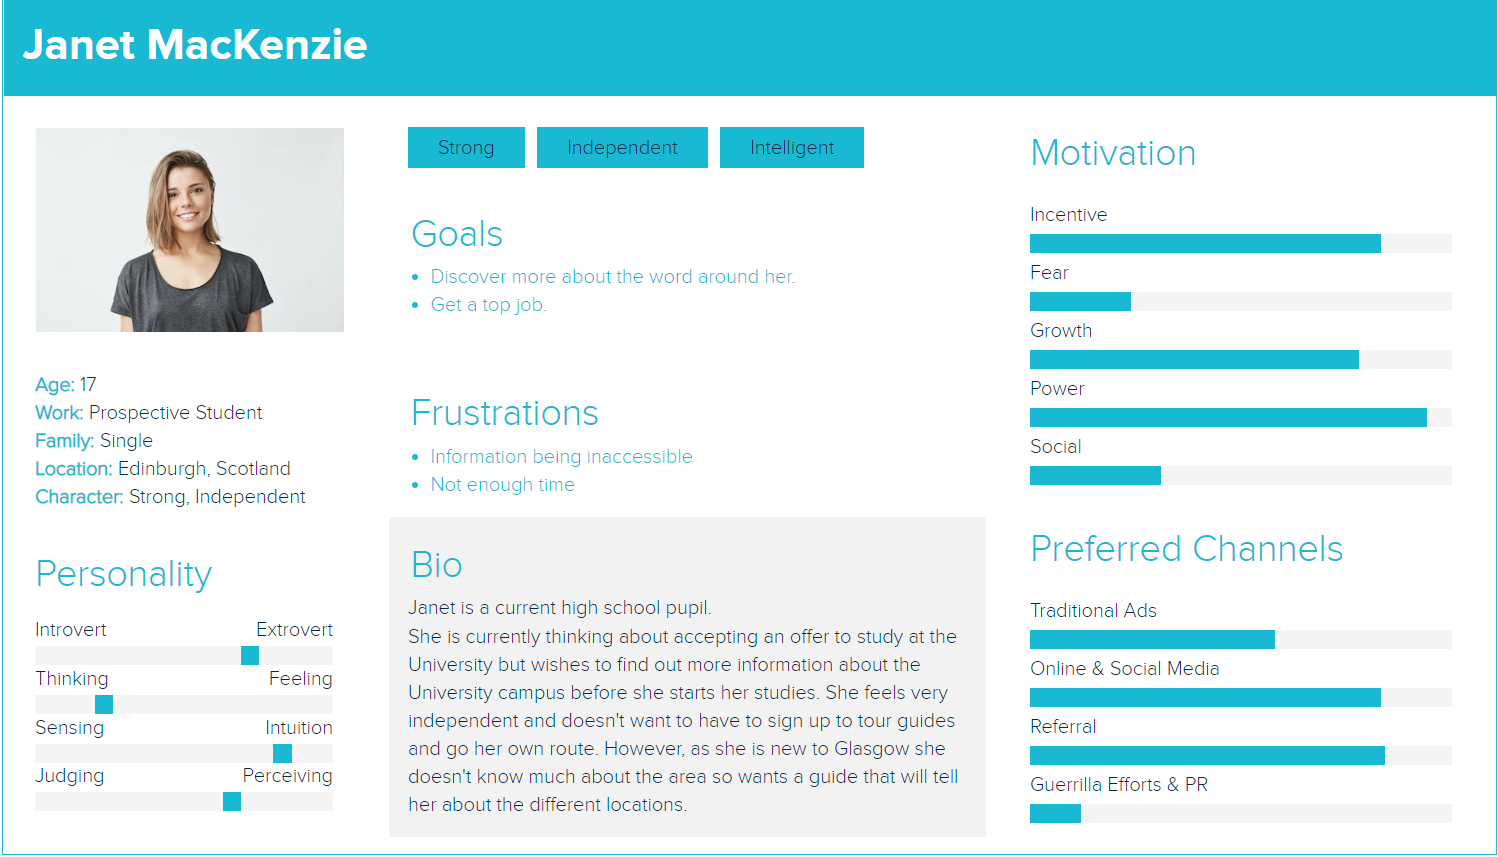
\includegraphics[width=1\columnwidth]{UserPersonaImage_Janet.PNG}
    \caption{User Persona - Janet MacKenzie}
    \label{fig:user1}
\end{figure}

\subsubsection{John Jack Jones}

John Jack, 22 years old, is currently studying Psychology at the University of Glasgow. He is looking for an application that he can use to learn more information about the campus around him and the buildings he uses. 

\begin{figure}[!h]
    \centering
    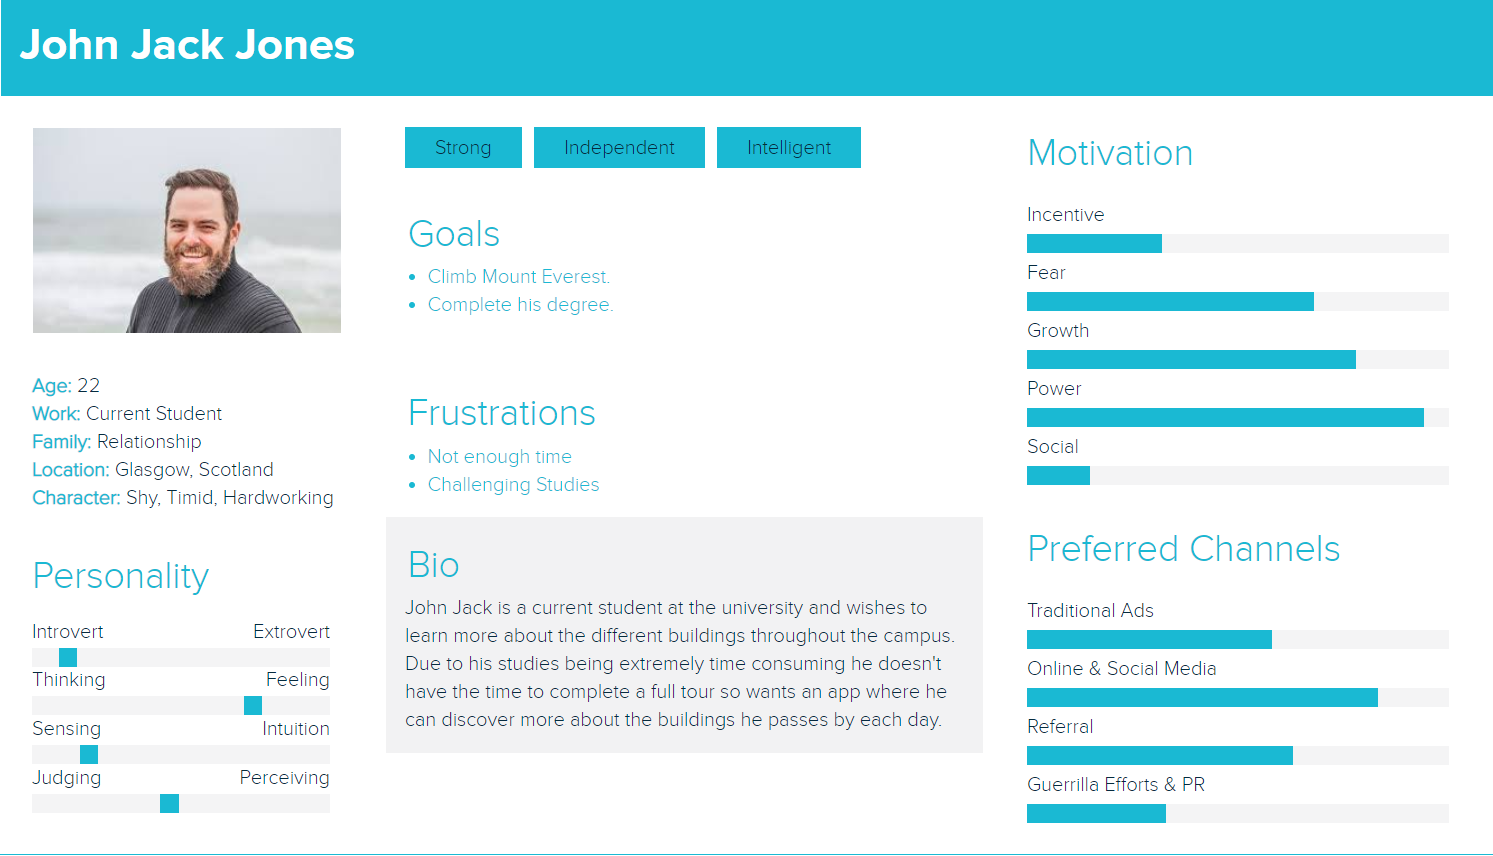
\includegraphics[width=1\columnwidth]{UserPersonaImage_John.PNG}
    \caption{User Persona - John Jack Jones}
    \label{fig:user2}    
\end{figure}

\subsubsection{Maggie Smith}

Maggie is a 72 year old woman, she is currently on holiday in Scotland. And wants to learn about the Universities famous buildings. However, she doesn't have the time in her itinerary to go on a guided tour so wants something quick and easy that will allow her and her friends to navigate around the buildings together. 

\begin{figure}[!h]
    \centering
    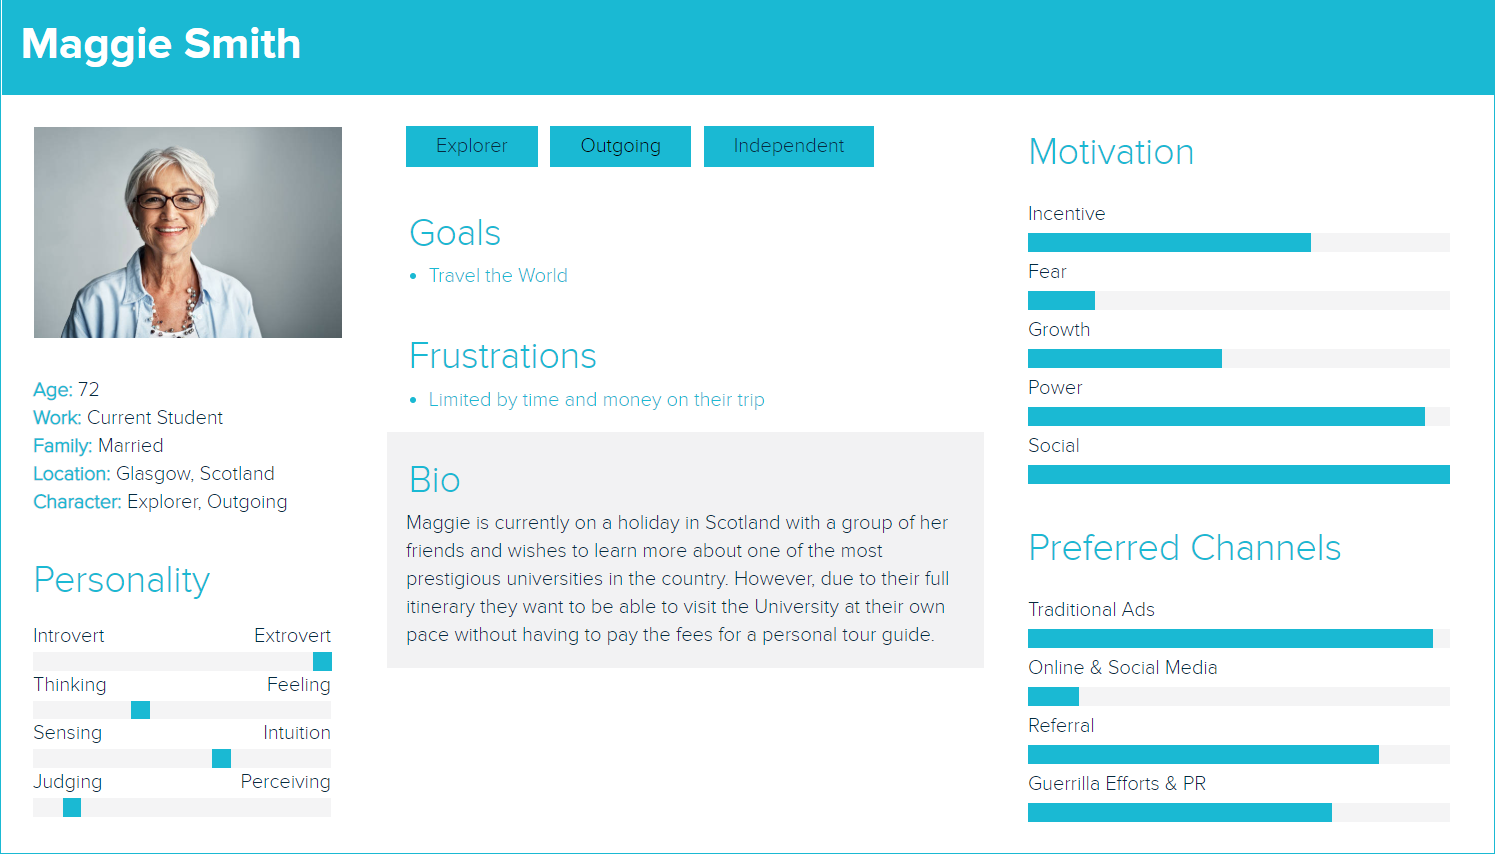
\includegraphics[width=1\columnwidth]{UserPersonaImage_Maggie.PNG}
    \caption{User Persona - Maggie Smith}
    \label{fig:user3}
\end{figure}

\subsection{Refined Requirements}
From our market research, we refined the original project requirements based on our responses. It was important to our target audience that the application was mobile based and ruled out wearable technology due to it not being accessible to every user. From section 4.2.4 results, we devised that our tour should be as fun and interactive as possible. We decided that the best course of action would be to gamify the app and make it as interactive as possible. From the last 2 questions, we discovered that it was imperative to users to have a map with in the tour app. In their feedback, they stated that it wouldn't make sense to have a tour guide app without a map as they would not know where to go. On top of this, we thought it would be good idea to have a friends feature which would encourage groups to use the app and interact with it together.

% ------------------------------------
\section{Concept Generation}
Within this section, we started the actual designing process for the application. These concepts were outlined by first generating an app definition statement. An app definition statement is a concise, concrete declaration of an app’s main purpose and its intended audience. We derived our app definition statement from our refined requirements.

\subsection{App Definition Statement}
Allow students, tourists and campus staff to discover more about the University of Glasgow and be able to find their way around the campus in a non-linear, interactive and free-form way. 
\newline
\newline
This app definition statement allowed us to generate initial concepts which are outlined below.

\subsection{Initial Ideas}
Using the research, our own imaginations and the generated App Definition Statement, we started drafting up potential concepts for the application. 

\subsubsection{QR-Code Scavenger Hunt}
The user presented with a list of ‘places of interest’ which are buildings or tourist spots around the campus. When the user sees a QR code around campus, they can scan it and it will display an information screen about the location. Once finished, reading the information, the user can mark the location as 'visited'. Visited locations are displayed as a map pin on a map. Game-like to collect all the locations, displays how many locations are left to find 

\subsubsection{Interactive App based on Geo-location}
User is presented with pictures of locations they can visit. When the user is within a certain radius of these locations, they can view information or get access to audio that will inform the user of information about that specific location and its history. Once the user has visited the location it will tick it off of the possible list of places to visit on the tour. The app adds an interactive element as the users are only presented with an image of the building and they need to try and find it just from that.

\subsubsection{Map Reveal App}
Users are initially presented with a blacked-out University campus map. As users discover and arrive at more places – these locations are unveiled, and additional information of each location is provided to the user. Once all locations are discovered the user will have access to bonus information about the University campus. 

\subsubsection{Hot and Cold Game}
Users are presented with a rough location of a QR code on a map. A scrambled image of the location of the QR code will initially be shown and it the user gets closer to the location the clearer the image becomes. Once the user arrives at the QR code they must scan the QR code and it will display information on that location. As the user walks away from the location the image will start to scramble again.

\subsubsection{Reflection}
From this we narrowed down to three ideas which we liked the best and best suited our user requirements. 

\subsection{Storyboards}
For the three application ideas we narrowed down to, we made a storyboard to depict their thought processes and further conceptualise how the application works in practice. These walked through a typical use case for the app with a user persona where the user navigates the app and completes the primary goals.

For our project we created storyboards for the following ideas;

Firstly, the QR-Code Scavenger Hunt, this storyboard depicts the users actions when using the application. Initially the user makes their way to a building which they haven't discovered yet. When they reach the building they must look around for the hidden QR Code, if the user is unable to locate it then they are able to ask for a hint. Upon discovering the QR code, the user can scan it using the in-app . camera. The app then displays information regarding that building to the user. And the location pin is added to the map so that the user may reference the building information later on. This can then be repeated until all the buildings are discovered.

Secondly, the Interactive App based on Geo-Location, this storyboard depicts a user initially at some random point on campus.The app will then display an image of a nearby building. The user must then look around the nearby buildings and head to the one shown in the image displayed. Once the user reaches the building an audio cue is played to indicate that they are at the correct building. The user can then scan the clearly displayed QR code and receive information about the building. The location of the building is stored on the users device allowing them to return to the information.

Finally, the Hot and Cold Game idea. This storyboard begins by showing the user a map containing pins of nearby points of interest. A scrambled image is displayed and as the user gets closer to the correct building the image becomes clearer. When the user finally arrives at the building they will be able to see the information regarding that building. This process is then repeated until the user has visited all the buildings of interest.

\subsection{Main Interaction concepts}

Our initial discussion entertained many different ways interaction with the app could be achieved. Suggestions included audio interaction, a video scavenger hunt, and using location data to find the nearest building for a user. It was decided to utilise QR Codes as our main interaction concept. These are common around the campus and many users will already be familiar with the concept. The clear advantage of using QR codes compared to other methods comes in the way they are accessed by the user. Having QR Codes in buildings around the campus allows the user to actively participate in the tour and explode their surroundings, instead of simply being delivered information through the app. It was argued that this active aspect of the tour would increase user satisfaction.


% ------------------------------------
\section{Initial Prototyping}

At this stage we took our narrowed down ideas and created a paper prototype of the User Interface for each one, as shown in Appendix \ref{app:proto}. We needed to take into consideration the preferences of our target audience outlined in Section 2. We tried to 

\subsection{Paper Prototypes}
Each team member created a paper prototype in order to encourage different ideas. These prototypes all centered around the QR Code technology that we agreed upon as the core of our application. They showcased the many different ways the technology can be harnessed and created a lot of discussion. In order to evaluate these varied ideas, the team conducted a discussion for each prototype, with members highlighting the advantages and disadvantages of each prototype.

These paper prototypes highlighted aspects of several dimensions of Interaction Design. All prototypes illustrated at least one aspect of Words, in the way of textual displays to the user in order to portray building information. Visual Representations are also used in the paper prototypes when display contextual information to the users, in 2/3 of the paper prototypes a floating action button was used to convey functionality to the user. The physical medium for each paper prototype was an Android phone. The interaction design of Time was not an aspect of any of the paper prototypes. Finally, Behaviour, the main behaviour of all the paper prototypes was to have a user scan a QR code and return values based off the code which was scanned. All the functionality of the application will be usable by a mobile application.

In order to evaluate the prototypes, the group discussed each of the designs in detail and highlighted pros and cons of different aspects within each of these. We also recruited, non-biased users to survey these paper prototypes and highlight their thoughts on different aspects of them.

From this, we decided to discard a few designs in our prototypes. Our prototypes' design was centered in the middle of the screen, with white space around the sides. This was dropped so that the whole screen was made available to be used with the application. The map view had to be refined, in order to display the full page as the map. Furthermore the help page was removed, as we felt it provided no functionality in the regards to the final application as users seemed to understand the design as easy-to-use and believed the help page would not provide any further clarity.

% ------------------------------------
\section{Refined Prototyping}
After creating a robust set of interaction designs that we prototyped and evaluated, we thought about how we could create a cohesive interactive experience using our individual concepts. We decided that digital wireframes would be the best way forward as they would give us a realistic idea of how our final would look and function.-

\subsection{Digital Wireframes}
Following our discussions, we decided to create our wireframes in Balsamiq. This would allow us to create a wireframe with some interaction, allowing users to navigate the app and progress between pages. The main page can be found in Figure \ref{fig:app} and the full wireframes can be found in Appendix \ref{app:refined}.

\begin{figure}[ht]
    \centering
    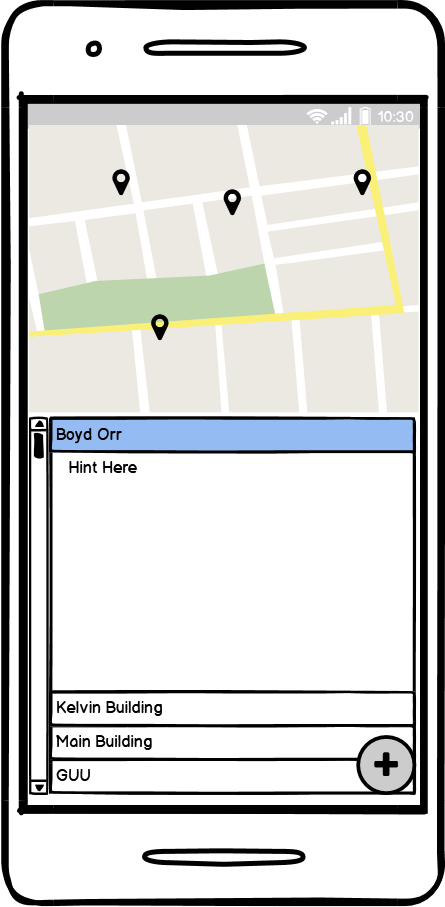
\includegraphics[width=0.5\columnwidth]{refinedPrototype4.png}
    \caption{Main page of Application}
    \label{fig:app}
\end{figure}

Main changes included the elimination of white space, allowing more room for the main app features and removal of the help page. 

\subsection{Evaluating Refined Prototype}

Through discussion of these wireframes, we concluded that the main page for our app should be the map, as it should be the core focus for users to see their collection of buildings. We also agreed that the building list should have a page of it's own, in order to include a picture of the building alongside it's name in the list, as users may not be sure of building names.

The team further discussed how to best provide navigation through the pages. Suggestions included a top or bottom navigation bar with icons for moving between all buildings, collected buildings and the main map screen. However, the final decision was to include a navigation drawer, accessible from swiping from the left of the screen to the right. This is a Android feature present in many apps and as a result, users will be familiar with this way to navigate the various pages in the app. This was also a requested feature from previous user surveys from Section \ref{bit:navbar}.

A team member raised the thought that the app did not do enough to encourage group activity, a design concept mentioned in the specification. This led to a discussion of how best to implement some kind of social feature. It was suggested to implement a Friends feature, that would allow users to add their friends through a username. Having users able to add friends and track what buildings their friends have scanned can introduce a social aspect that encourages the use of the app and possibly even some competitiveness between users to 'collect' all the buildings before their friends.

The team also performed User evaluations on the refined prototypes using the think aloud method. Where we got participants to navigate through the Balsamiq prototypes, and the tester would ask four different questions throughout the walk through of the application; What are you thinking? What are you trying to do? Do you have any questions about the app? and What do you like / dislike and how can we improve the design?.

Following this evaluation we discovered multiple areas within the app which needed to be improved, changed or kept. 
Firstly, one of the main concerns of both participants was the lack of navigational clarity within the application. At several points throughout both think aloud evaluations the users became unsure of how to proceed in the app to the next logical page. 
Another point made by both participants concerned the overall design of the application. On one hand, participant 1 liked the design whereas participant 2 did not, as we want to try and create an app suitable and enjoyable for everyone, it is up to the team to create an app that finds a suitable medium between these contrasting views. 
Both users completed the task of locate the building information successfully which is very positive sign regarding the usability of our refined prototypes of the application. 
Finally, both users also really liked the idea of the application and thought it was new and an exciting prospect that they would use if it was released.

% ------------------------------------
\section{Final Prototype}
The final prototype is the culmination of all previous refinement stages. We evaluated these stages, listened to all our user feedback and from this our final prototype was born.

\subsection{Validity of Initial Ideas}
While the implementation has changed throughout development, the initial essence of the app remains the same - a tour of the University, delivered primarily through encouraging searching for QR Codes featured in each building on campus. The application encourages social cooperation in the tour by helping others 'collect' the buildings around campus. This is further emphasised by a friend system where you can see your friends' progress in the tour. 

\subsection{Android Studio App}
Our final application was developed using Android Studio as all of the team members were familiar with the environment and its components. The components used within our application are generic to Android. We decided to use these components because it would mean that users would be able to easily use and navigate our app without a technical person showing them how to use it. We wanted to ensure that users were able a navigate through the app with absolutely no issues. We did this through the use of a navigation drawer.

\subsection{Implementation}
In our refined wireframes, we did not have a any form of navigation bar which was an overlook on our behalf. At first, we did not think it would be necessary and thought the app would be able to navigate the user through it automatically. After careful consideration, we decided that this was not the best approach as the user would have no way of getting to other pages by themselves. Using the think aloud method, we received feedback that the the application was hard to navigate - this was our main reason for adding navigation to the app. We implemented this in the form of a navigation drawer which is accessible to the user from most pages. On top of this, we added pages which allows the user to see which buildings they have visited and also a list of all locations which act as a hint for buildings that they can discover. A friends page has has also been added as in the original project specification, it states that the we should design an app that can be enjoyed by a group of people. In our wireframes, we had not considered this requirement and what the best way to implement it would be. However, after discussion, a simple friends feature was decided as the best system to deliver a social experience. The friends page allows users to add friends and see which buildings that they have discovered.

% ------------------------------------

\subsection{App Screenshots}

\begin{figure}[!h]
    \centering
    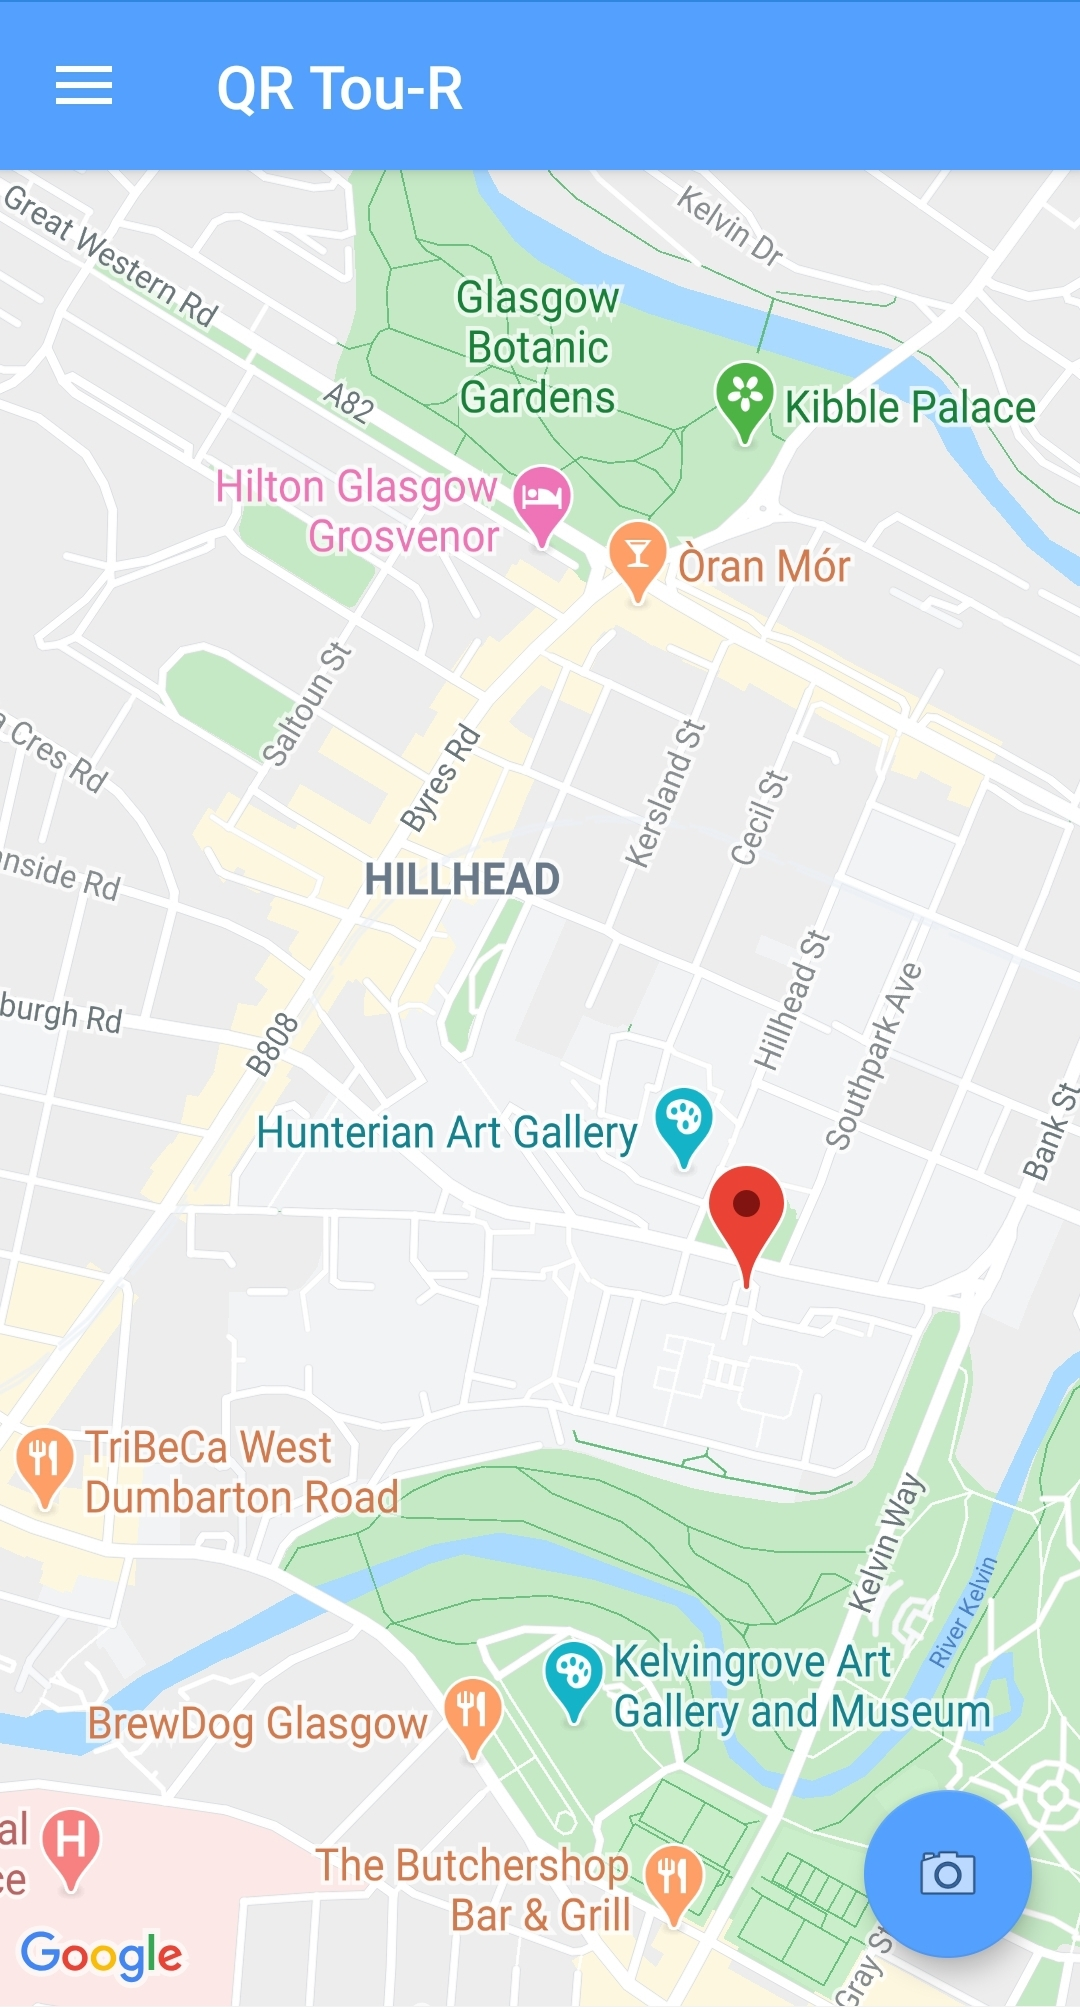
\includegraphics[width=0.4\columnwidth]{app1.jpg}
    \caption{Main map page of Final Prototype}
    \label{fig:appfinalmain}
\end{figure}

\begin{figure}[!h]
    \centering
    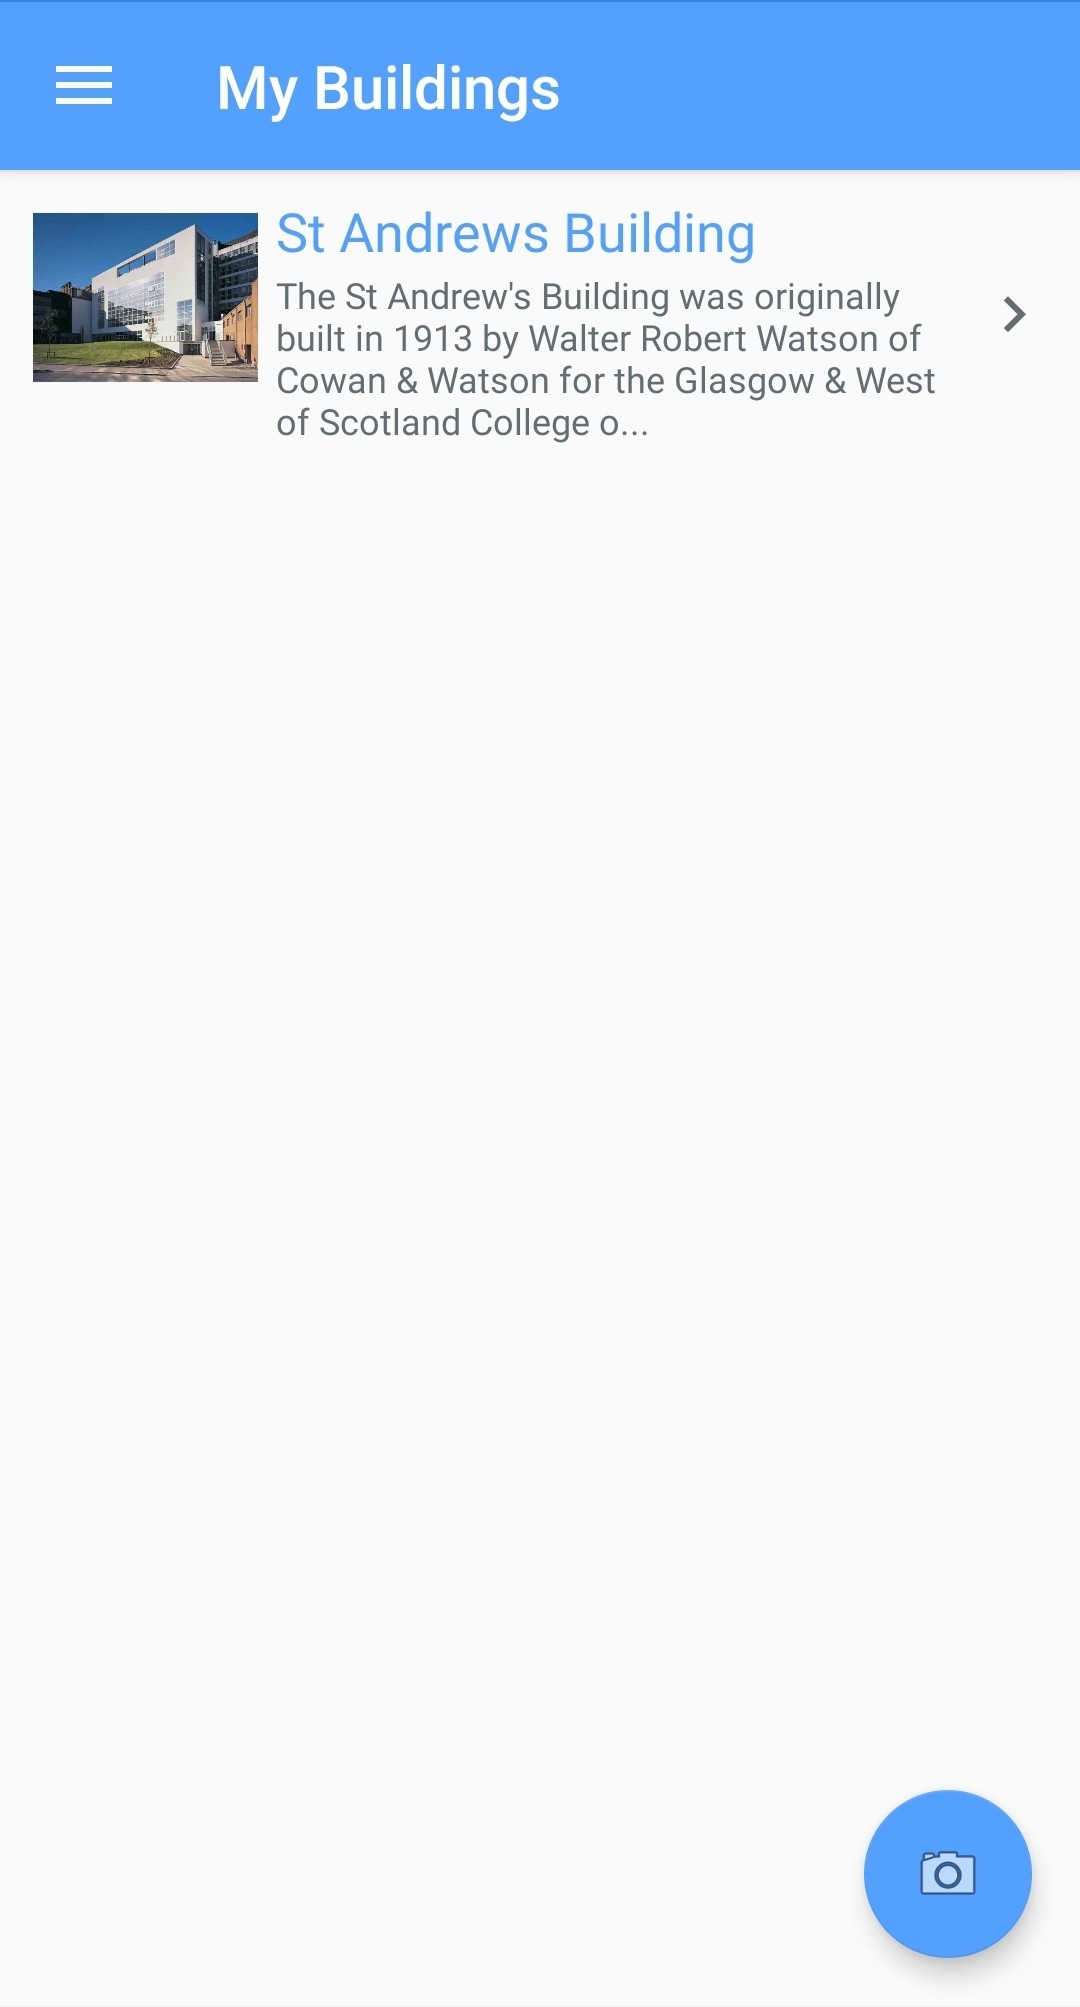
\includegraphics[width=0.4\columnwidth]{app6.jpg}
    \caption{My Buildings Page}
    \label{fig:appfinalmain}
\end{figure}

\begin{figure}[!h]
    \centering
    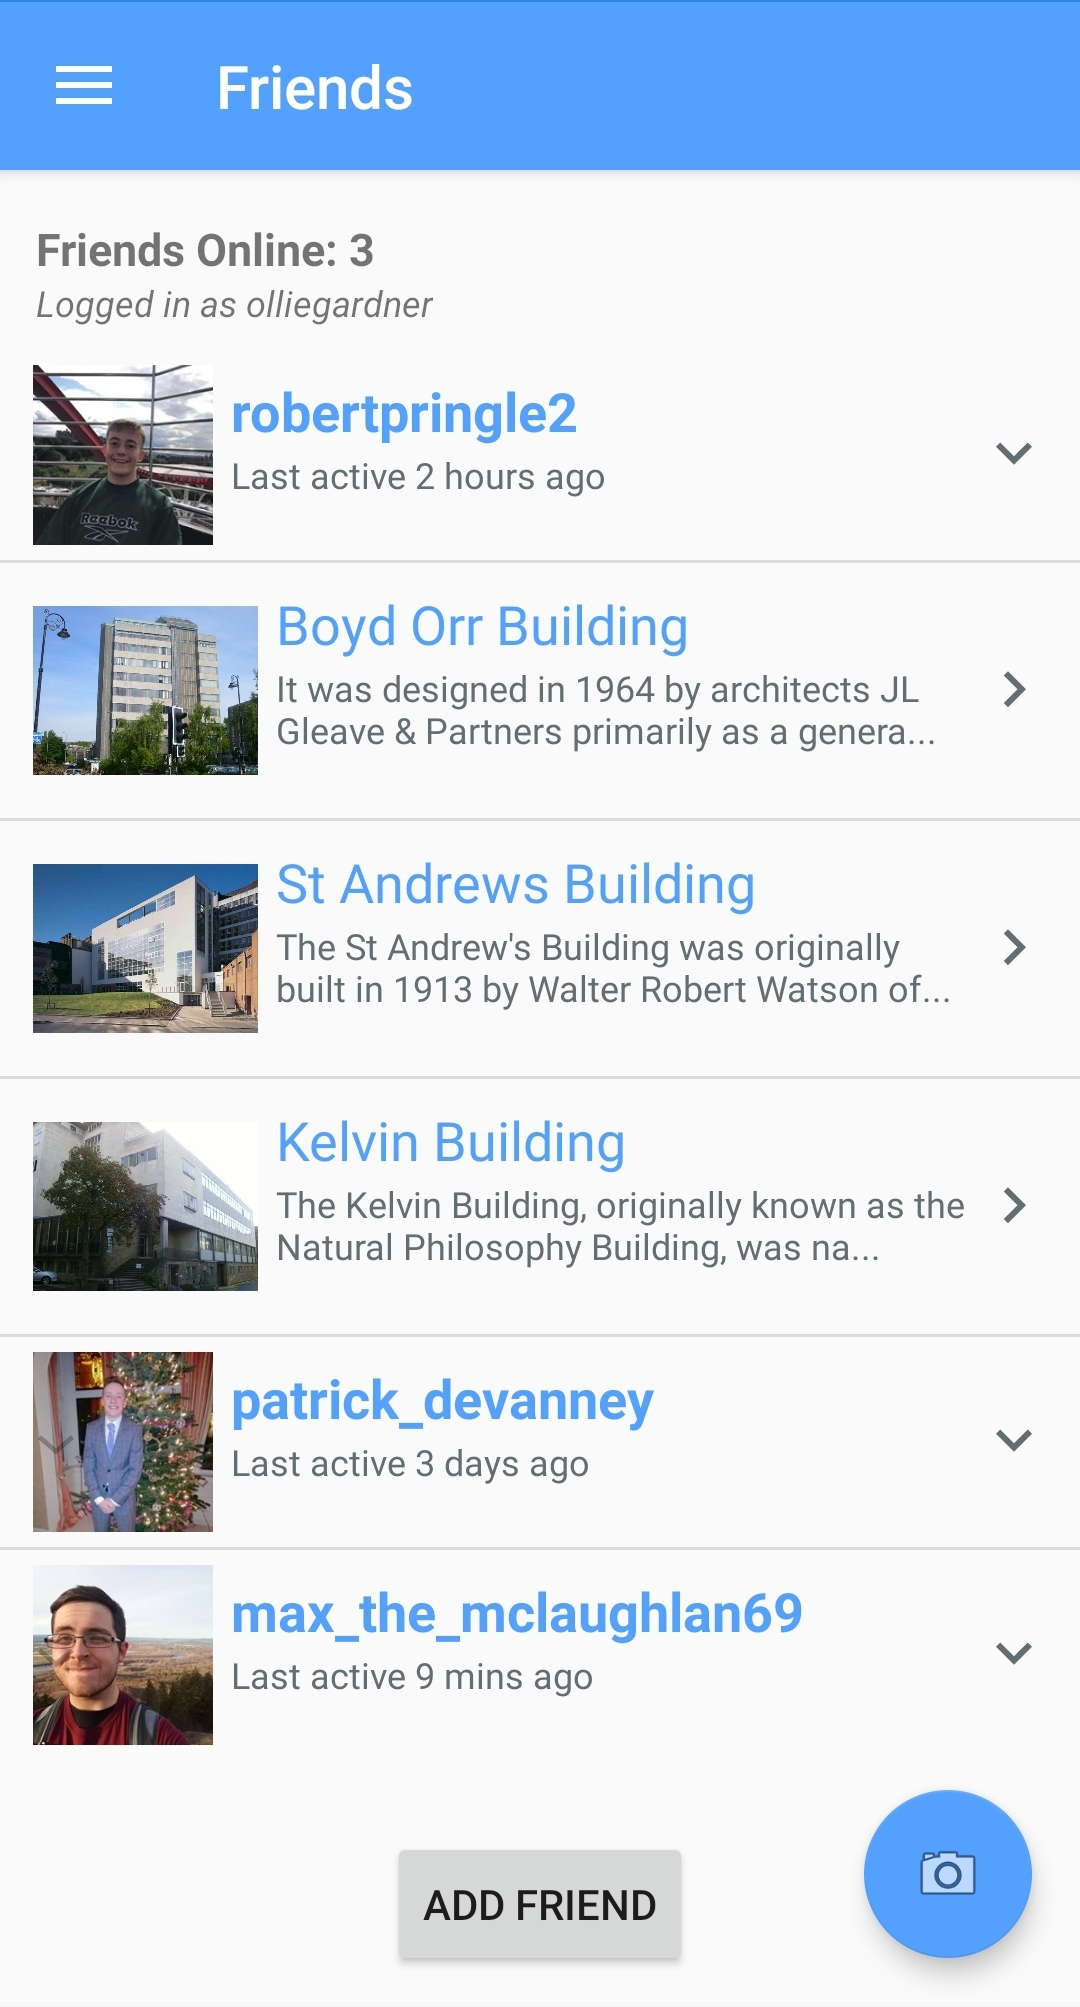
\includegraphics[width=0.4\columnwidth]{app3.jpg}
    \caption{Friends page with friends' buildings}
    \label{fig:appfinalmain}
\end{figure}

\begin{figure}[!h]
    \centering
    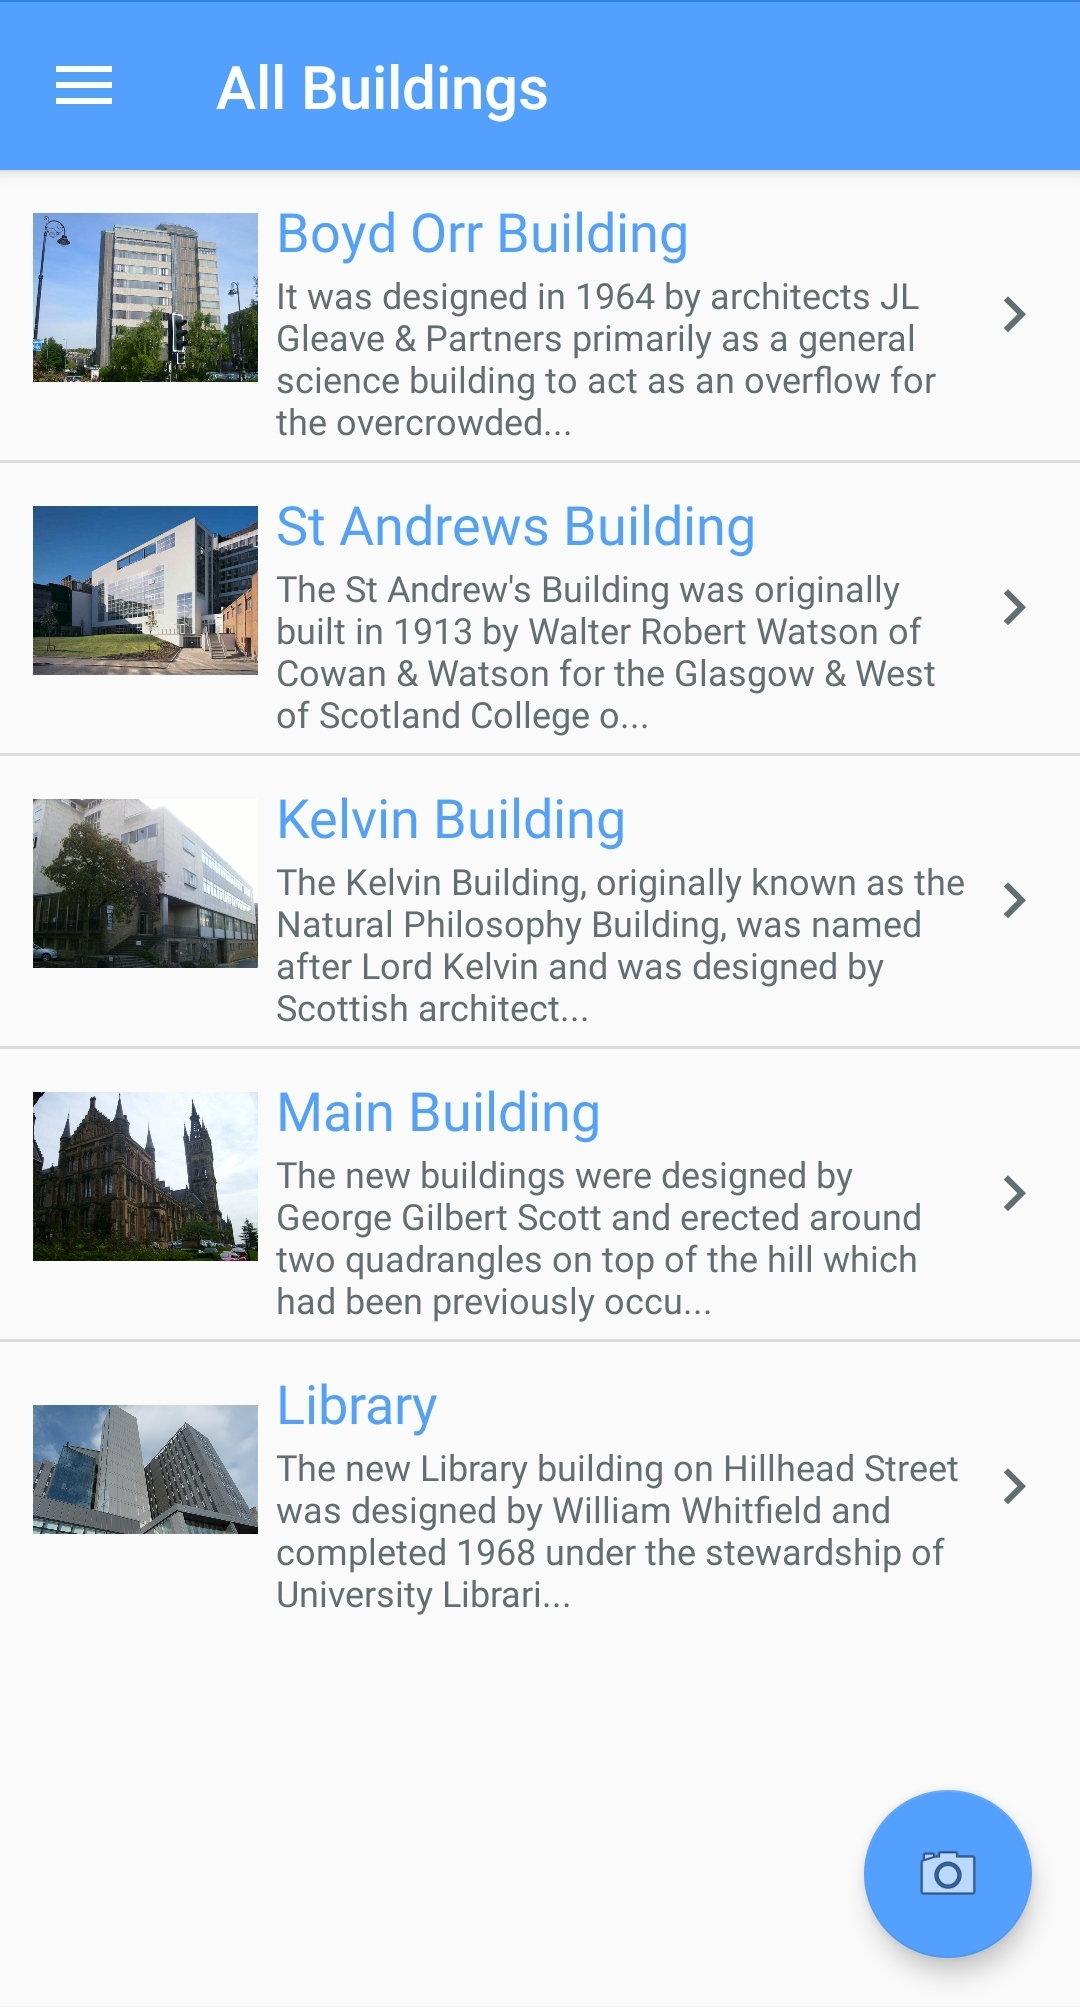
\includegraphics[width=0.4\columnwidth]{app4.jpg}
    \caption{Page listing All Buildings}
    \label{fig:appfinalmain}
\end{figure}

\begin{figure}[!h]
    \centering
    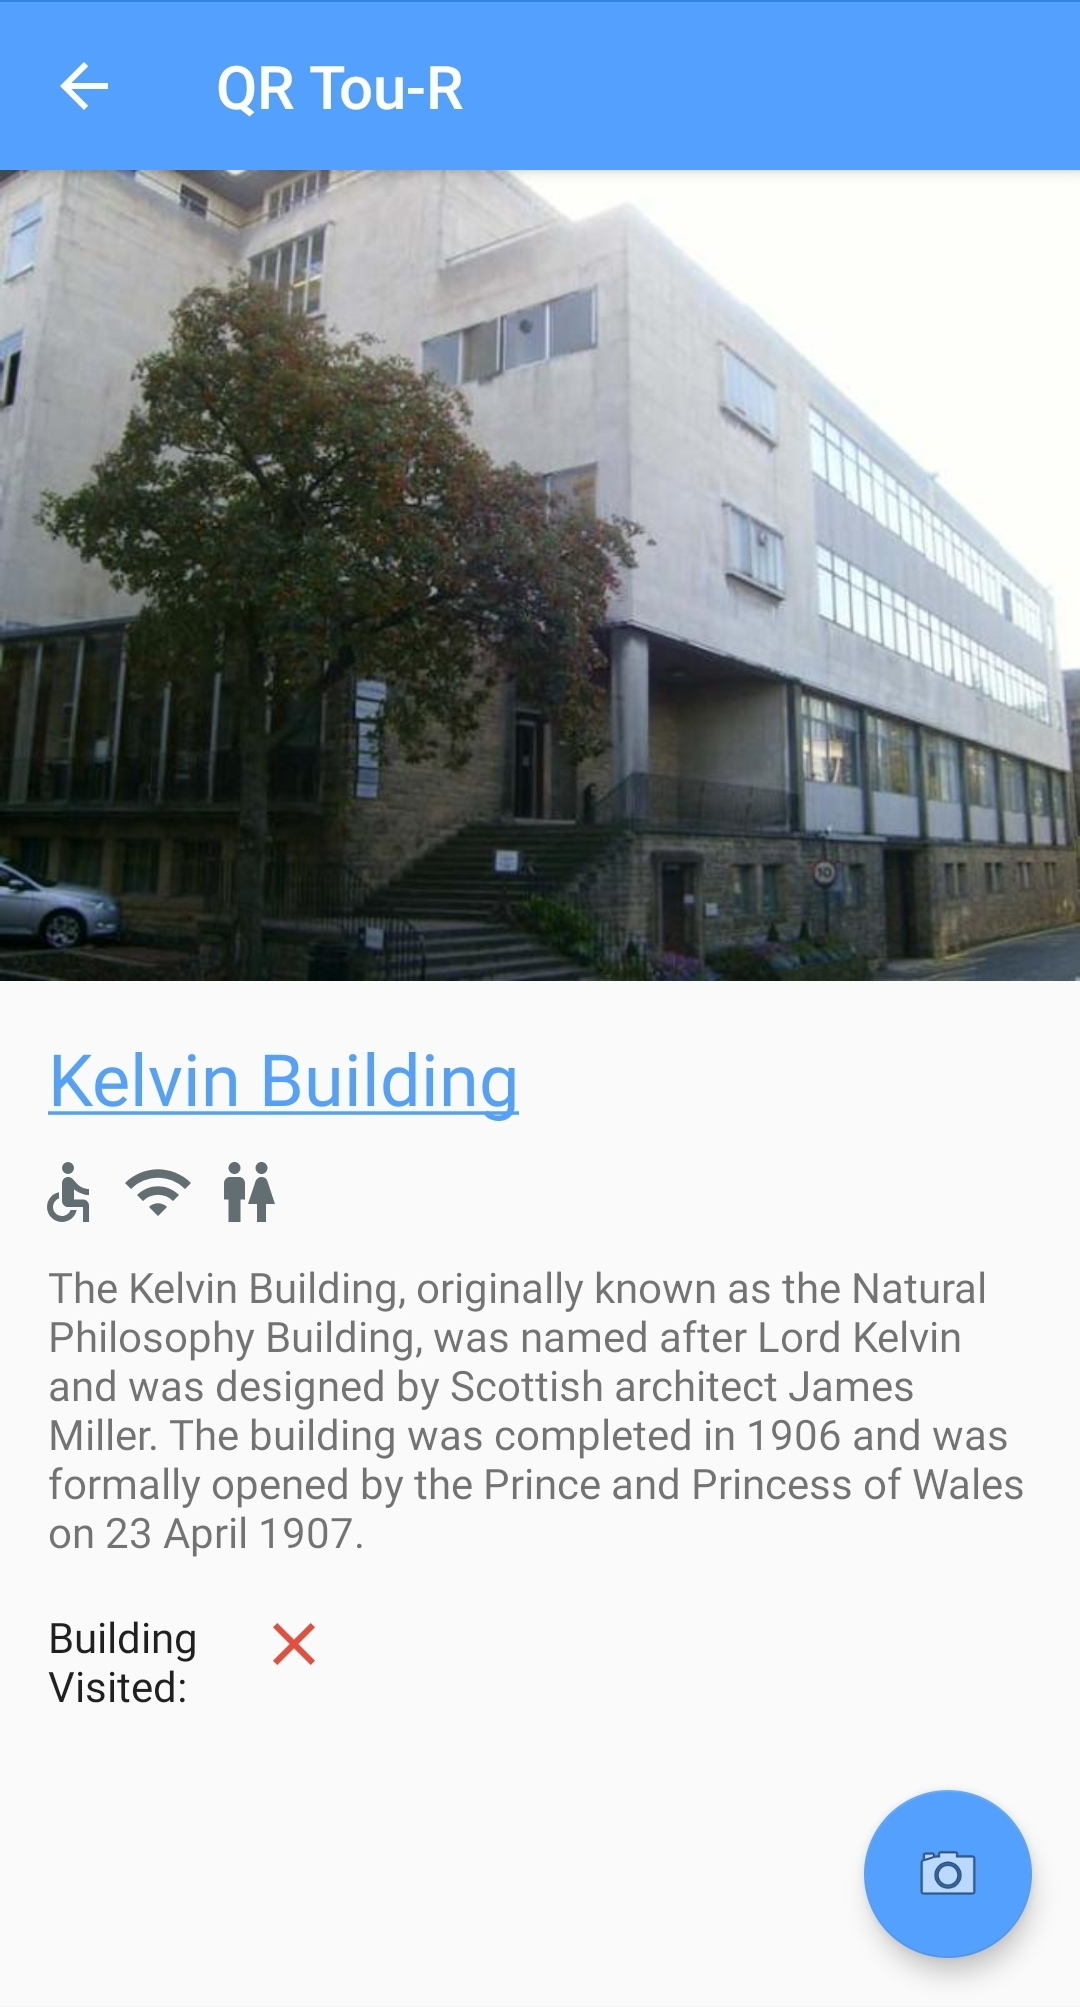
\includegraphics[width=0.4\columnwidth]{app5.jpg}
    \caption{Page showing building information}
    \label{fig:appfinalmain}
\end{figure}

\newpage

\subsection{Evaluation}
For the evaluation we are making use of the SUS survey which measures agreement with statements about usability. The survey  consists of ten questions, shown in appendix \ref{appen:eval}. We chose eight participants studying computing experience. Before our eight participants filled the survey in, we explained the application idea to them and let them use the application on a phone. We let them use it for about a five minute time period to familiarize themselves with the application.

\subsubsection{Question 1}
\noindent\emph{I think that I would like to use this system frequently.}
\newline
\newline
Four of the users said they were neutral and the other four said they would not like to use the application frequently. This can be expected as users usually will not frequently participate in the same tour over and over again.

\subsubsection{Question 2}
\noindent\emph{I found the system unnecessarily complex.}
\newline
\newline
All users strongly disagreed that the system was unnecessarily complex. This is good as it showed we kept our design simple enough to easily understand how to interact with it.

\subsubsection{Question 3}
\noindent\emph{I thought the system was easy to use.}
\newline
\newline
Six of our participants said here they strongly agree that the system was easy to use. However one participant said they disagree and an other said they strongly disagree with this statement. It is encouraging that the majority of users found it easy to use, but we need to take all users into consideration. The two users who disagreed may have less experience using mobile applications or have their own limitations that does not allow them to easily interact with the application (e.g. a disability).

\subsubsection{Question 4}
\noindent\emph{I think that I would need the support of a technical person to be able to use this system.}
\newline
\newline
5/8 participants Strongly Disagreed that they would need the support of a technical person to use the system. This suggests that focusing on a familiar, user-friendly design resulted in an application that can be used with ease by a varied group of users. 

\subsubsection{Question 5}
\noindent\emph{I found the various functions in this system were well integrated.}
\newline
\newline
4/8 participants either Agreed or Strongly Agreed with the statement 'I found the various functions in this system were well integrated'. Only one participant Strongly Disagreed with this statement. From this, we can assume that users on the whole are happy with the way the primary functions - the QR Code building collecting and Friends feature - were well integrated and work well together. 

\subsubsection{Question 6}
\noindent\emph{I thought there was too much inconsistency in this system.}
\newline
\newline
7/8 participants in the study Disagreed or Strongly Disagreed that 'I thought there was too much inconsistency in this system.' We can conclude that the final design was consistent across the pages in the app, with a similar layout and colour scheme across pages helping users feel that each page flows from one to another in a satisfying way. 

\subsubsection{Question 7}
\noindent\emph{I would imagine that most people would learn to use this system very quickly.}
\newline
\newline
A majority of users (5/8) believed that the system would be easy to learn for most people. This is encouraging, as many users who download the app to tour the campus may not have English as a first language. The minimal use of language within the app - other than building descriptions - aims to encourage the user to explore the different pages of the app at their own pace and in their own way. 

\subsubsection{Question 8}
\noindent\emph{I found the system very cumbersome to use.}
\newline
\newline
4/8 participants Strongly Disagreed that they found the system cumbersome to use. This may be due to the minimal number of different pages in the app, keeping it as simple as possible. The consistent design for each building page ensures that users will know what layout to expect for each building. 

\subsubsection{Question 9}
\noindent\emph{I felt very confident using the system.}
\newline
\newline
Half of the users said they strongly agreed that they were confident using the system, three said they agreed and one said they disagreed. Since the majority of the users had a positive response it suggests to us that most people would be confident using the system. Again, since now all people are experienced using mobile applications and we tried to evaluate users with a wide variety of experience it can be expected to get someone to disagree with this statement.

\subsubsection{Question 10}
\noindent\emph{I needed to learn a lot of things before I could get going with this system.}
\newline
\newline
One participant said that they agree that they would need to learn a lot of things before they could get used to the system. This is contradictory to the general response as the rest of the participants said they strongly disagree with the same statement. This shows our application generally does not require you to learn new things to work it. The one person who thought they did might not be an experienced user with mobile applications o have some sort of impairment limiting them to interact with the application as intended.

% ------------------------------------
\section{Conclusion}
QR Tou-R started with a simple of idea of providing people with an innovative and interactive modern tour guide experience. Through working through mobile application development methods, we have successfully implemented a strong prototype which meets our defined requirements. 

Evaluation was carried out at multiple stages in the development process, allowing us to refine the design and layouts to meet user recommendations. This iterative design process let us effectively test initial design ideas in order to discard poorer layouts and improve upon the best ones. 

The positive feedback from the evaluation of our final prototype has led us to believe the application would be successful as a product. Specifically, the "collecting" focus of the tour allowing the user to go at their own pace and see their friends progress, was well received.

% ------------------------------------
\begin{thebibliography}{9}
\bibitem{guidedtour} 
\texttt{https://www.gla.ac.uk/explore/visit/attraction
s/guidedtour/}

\bibitem{wehostanytour} 
\texttt{https://www.wehostanytour.com/}

\bibitem{gpsmycity} 
\texttt{https://www.gpsmycity.com/}
\end{thebibliography}

\clearpage
\newpage

% ------------------------------------
\section{Appendix}
Please find here supplementing information referenced in the report.

\subsection{Market Research}
\label{res:quest}
\noindent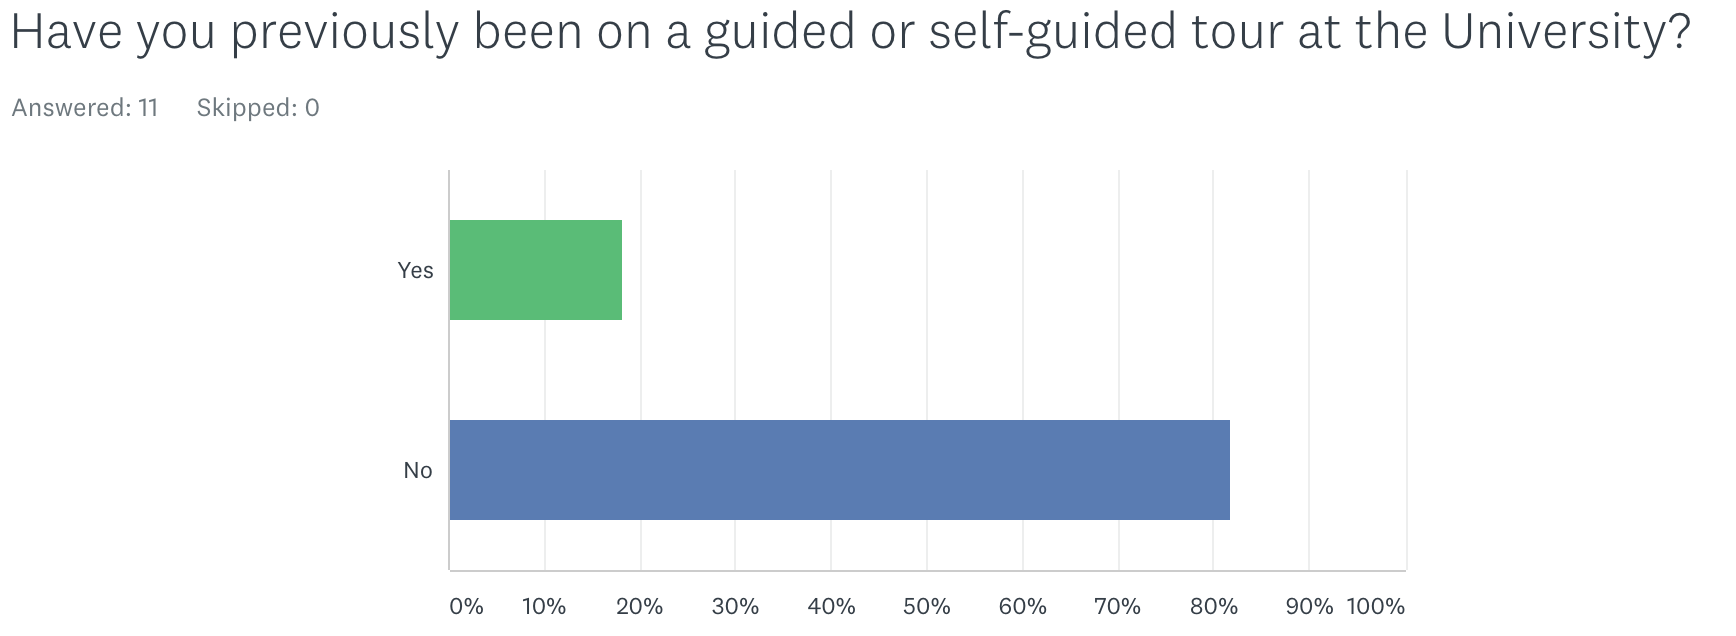
\includegraphics[width=\columnwidth]{Question1.png}
\noindent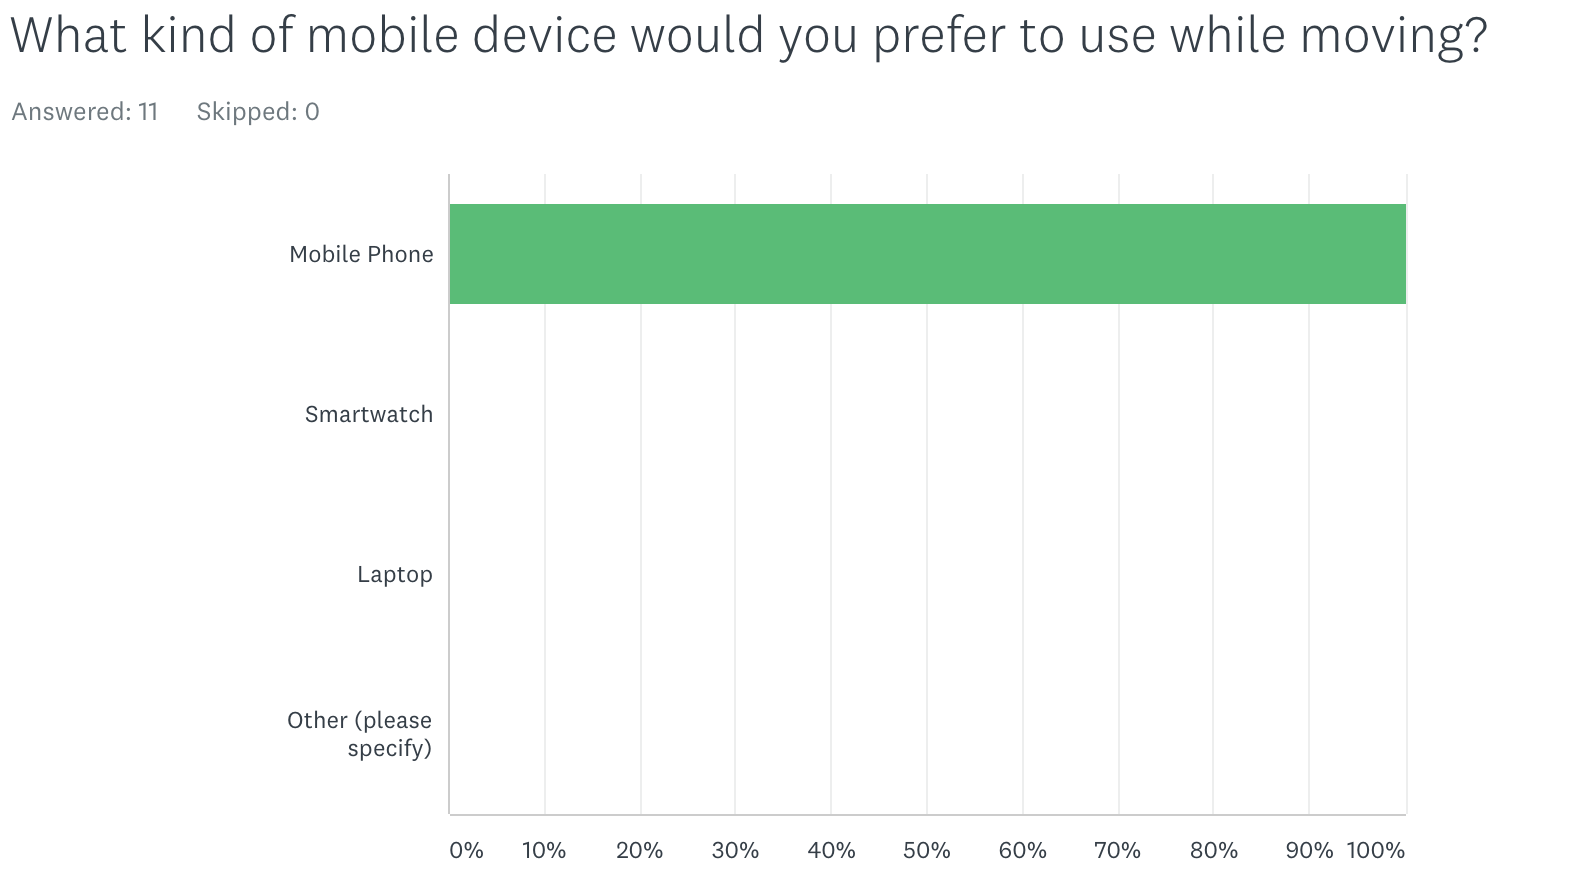
\includegraphics[width=\columnwidth]{Question3.png}
\noindent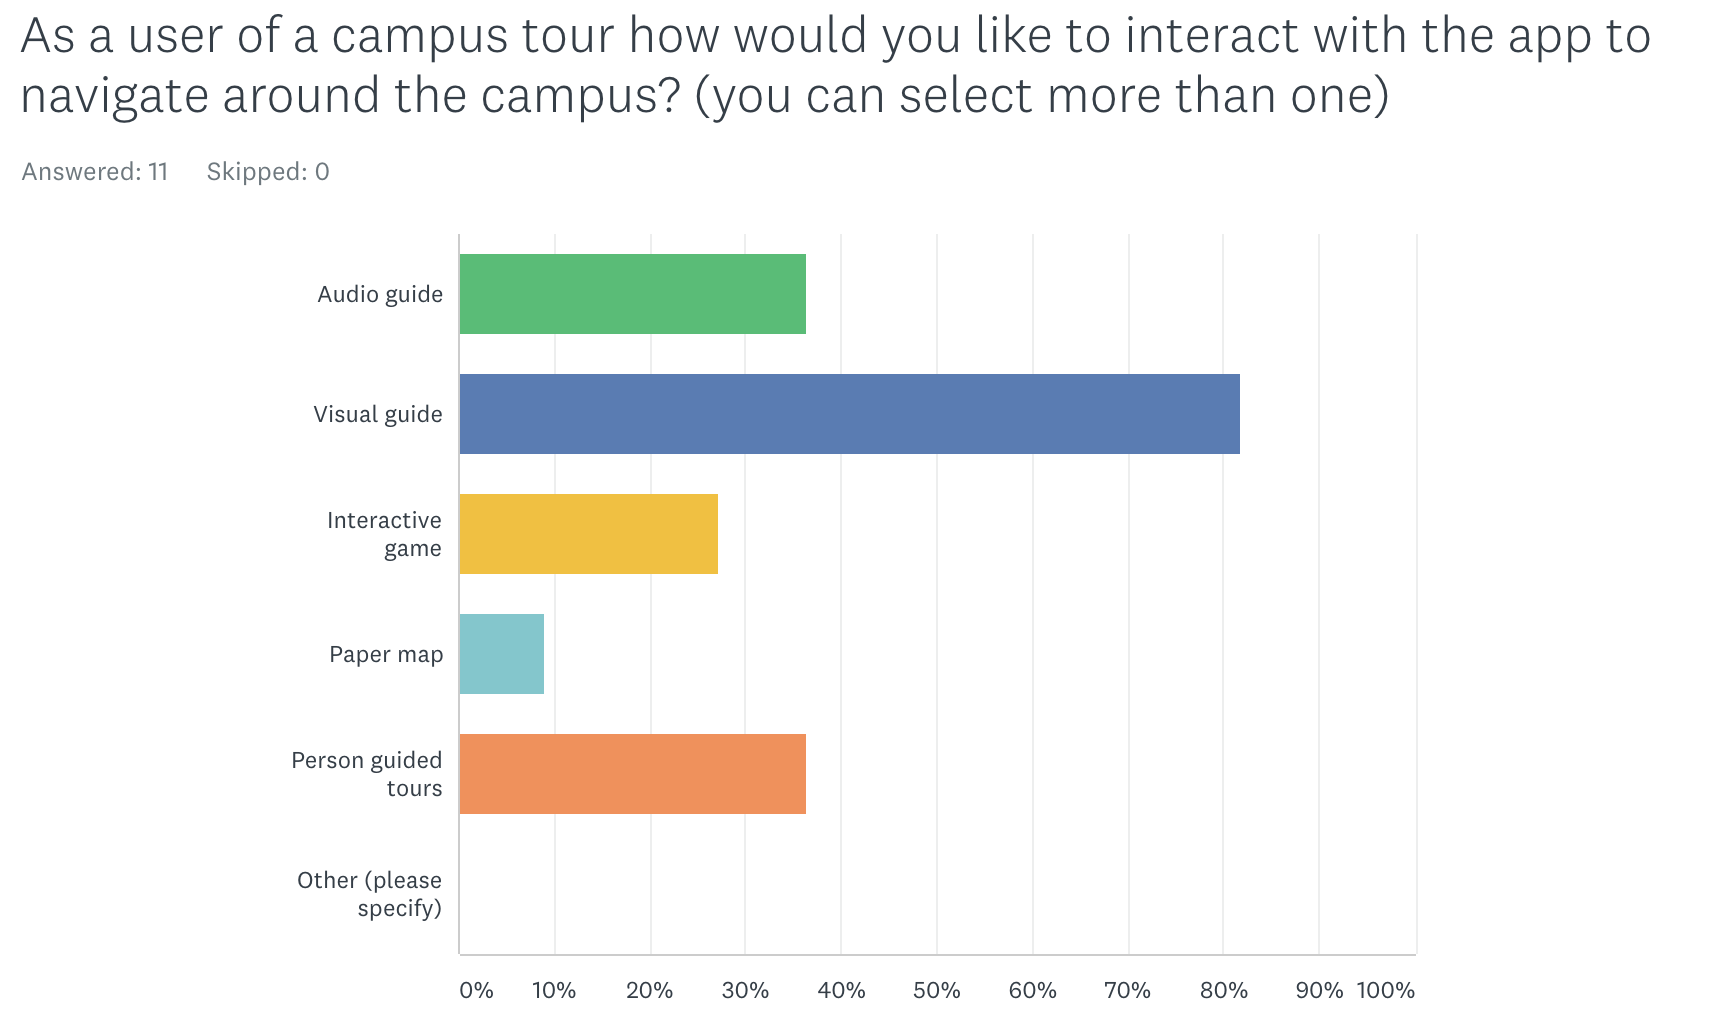
\includegraphics[width=\columnwidth]{Question5.png}
\noindent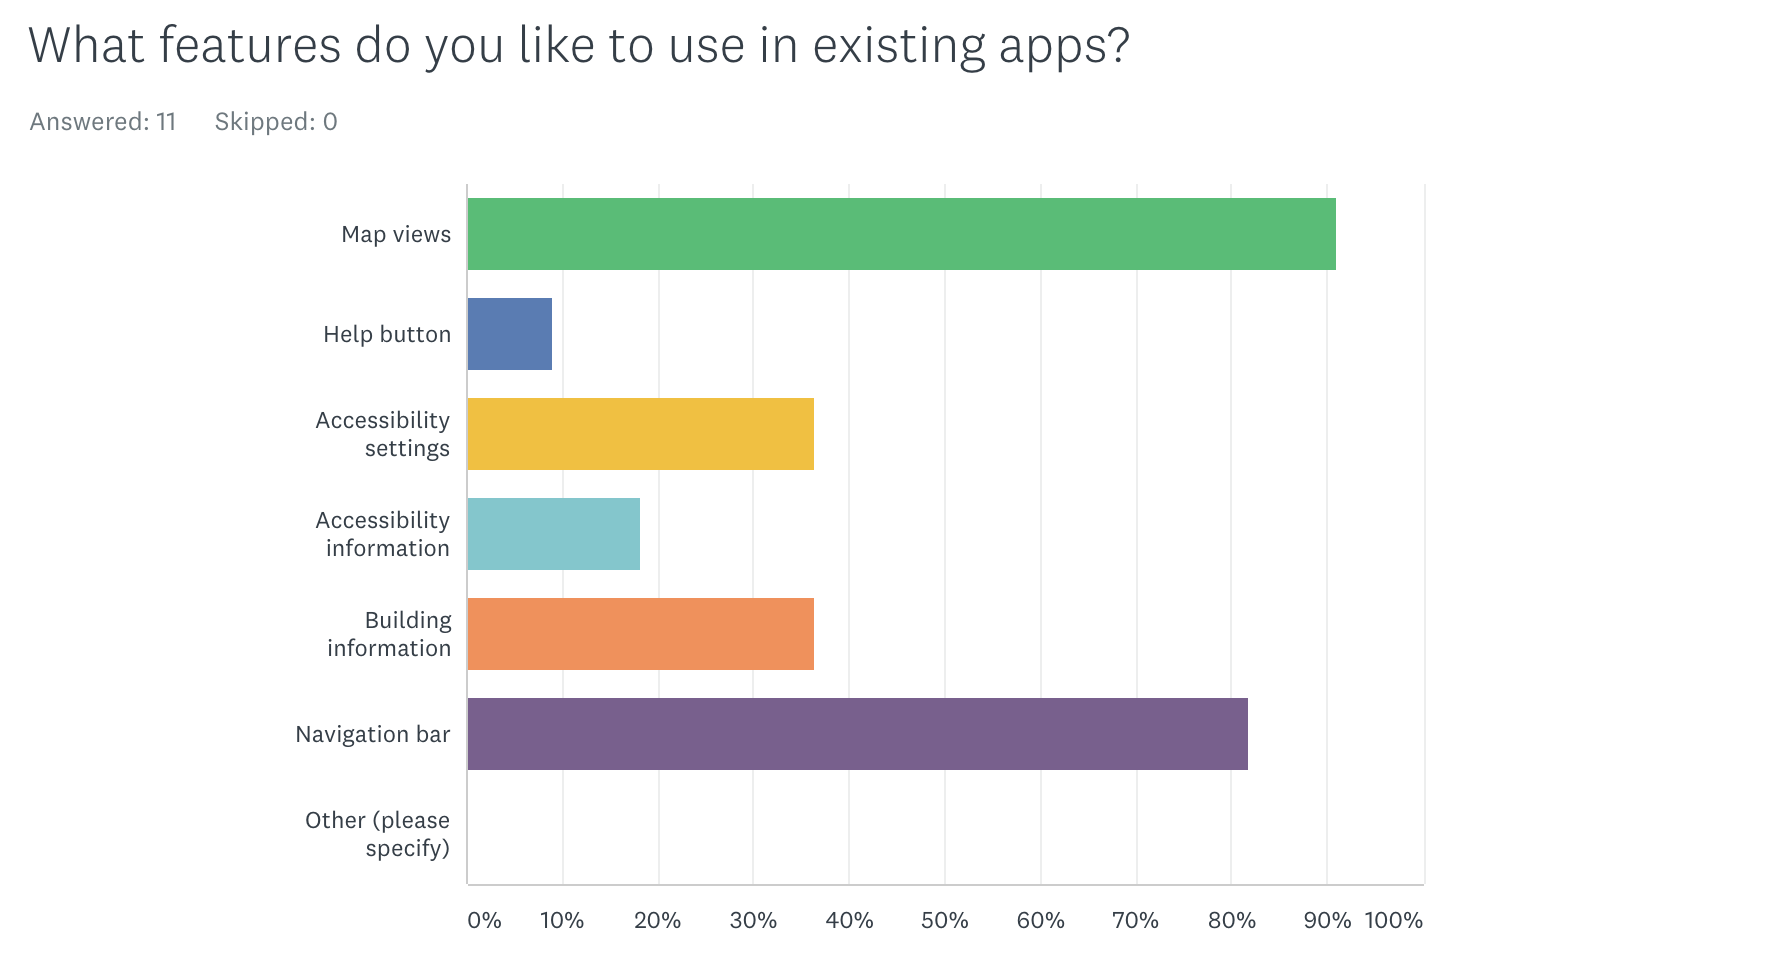
\includegraphics[width=\columnwidth]{Question6.png}

\subsection{Storyboards}
\label{app:storyboards}
\noindent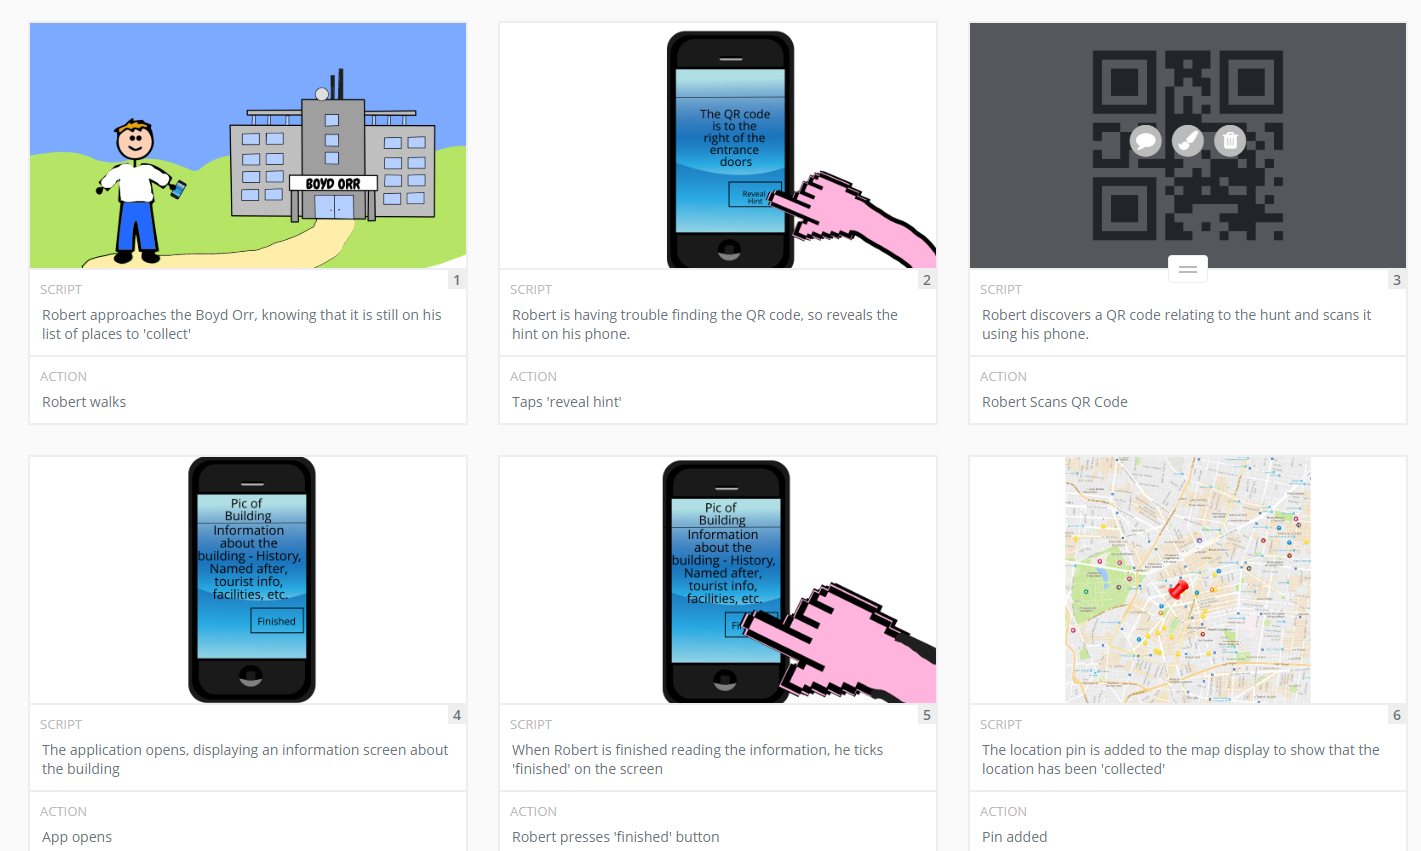
\includegraphics[width=\columnwidth]{storyboard1.PNG}
\noindent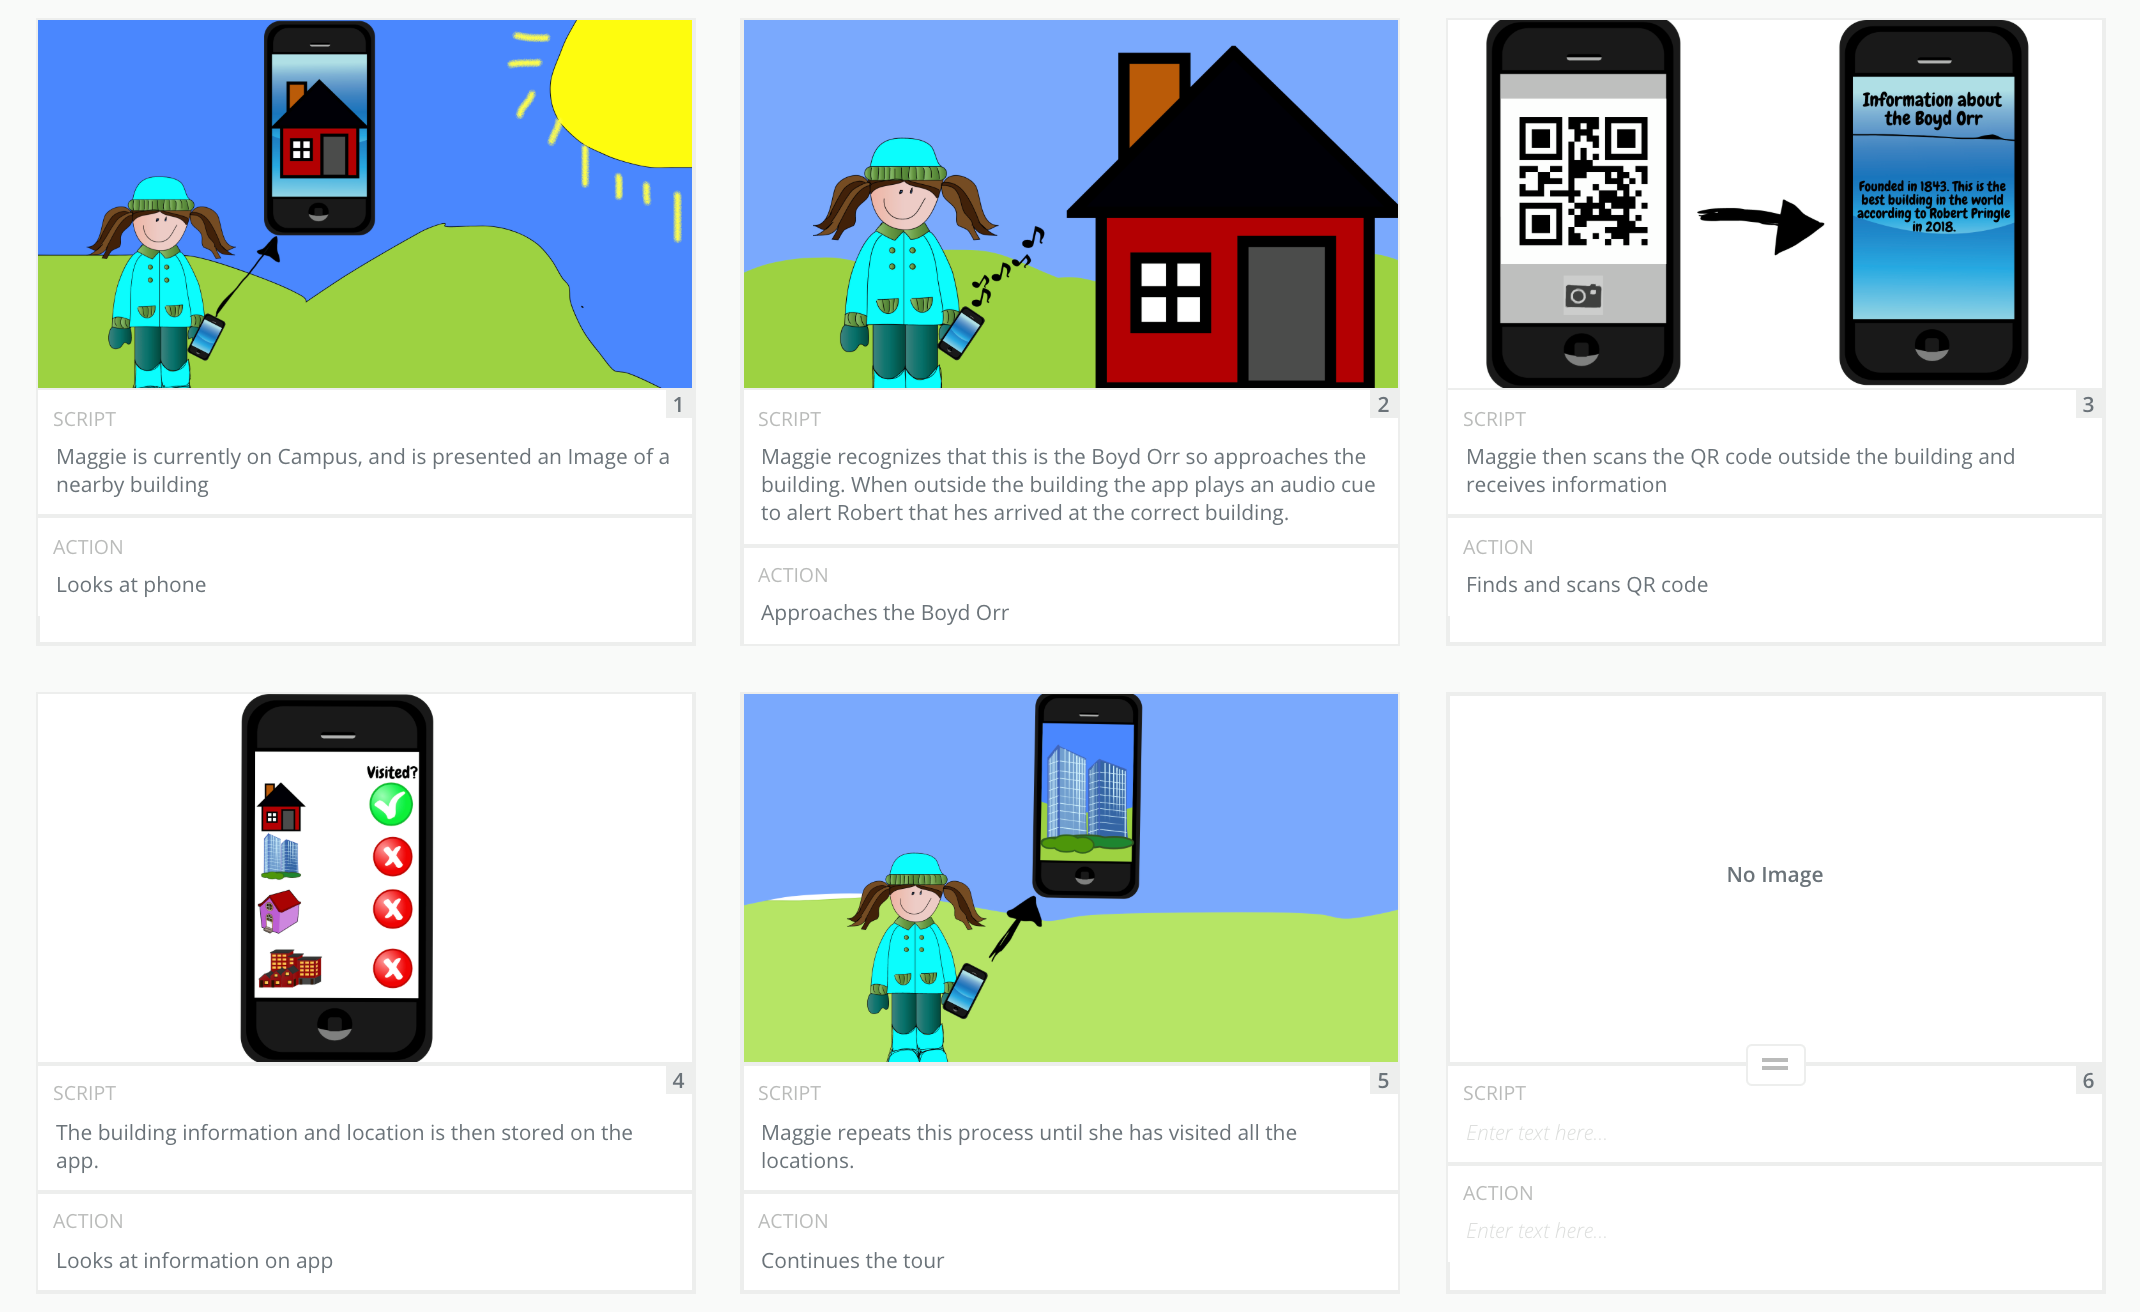
\includegraphics[width=\columnwidth]{storyboard2.png}
\noindent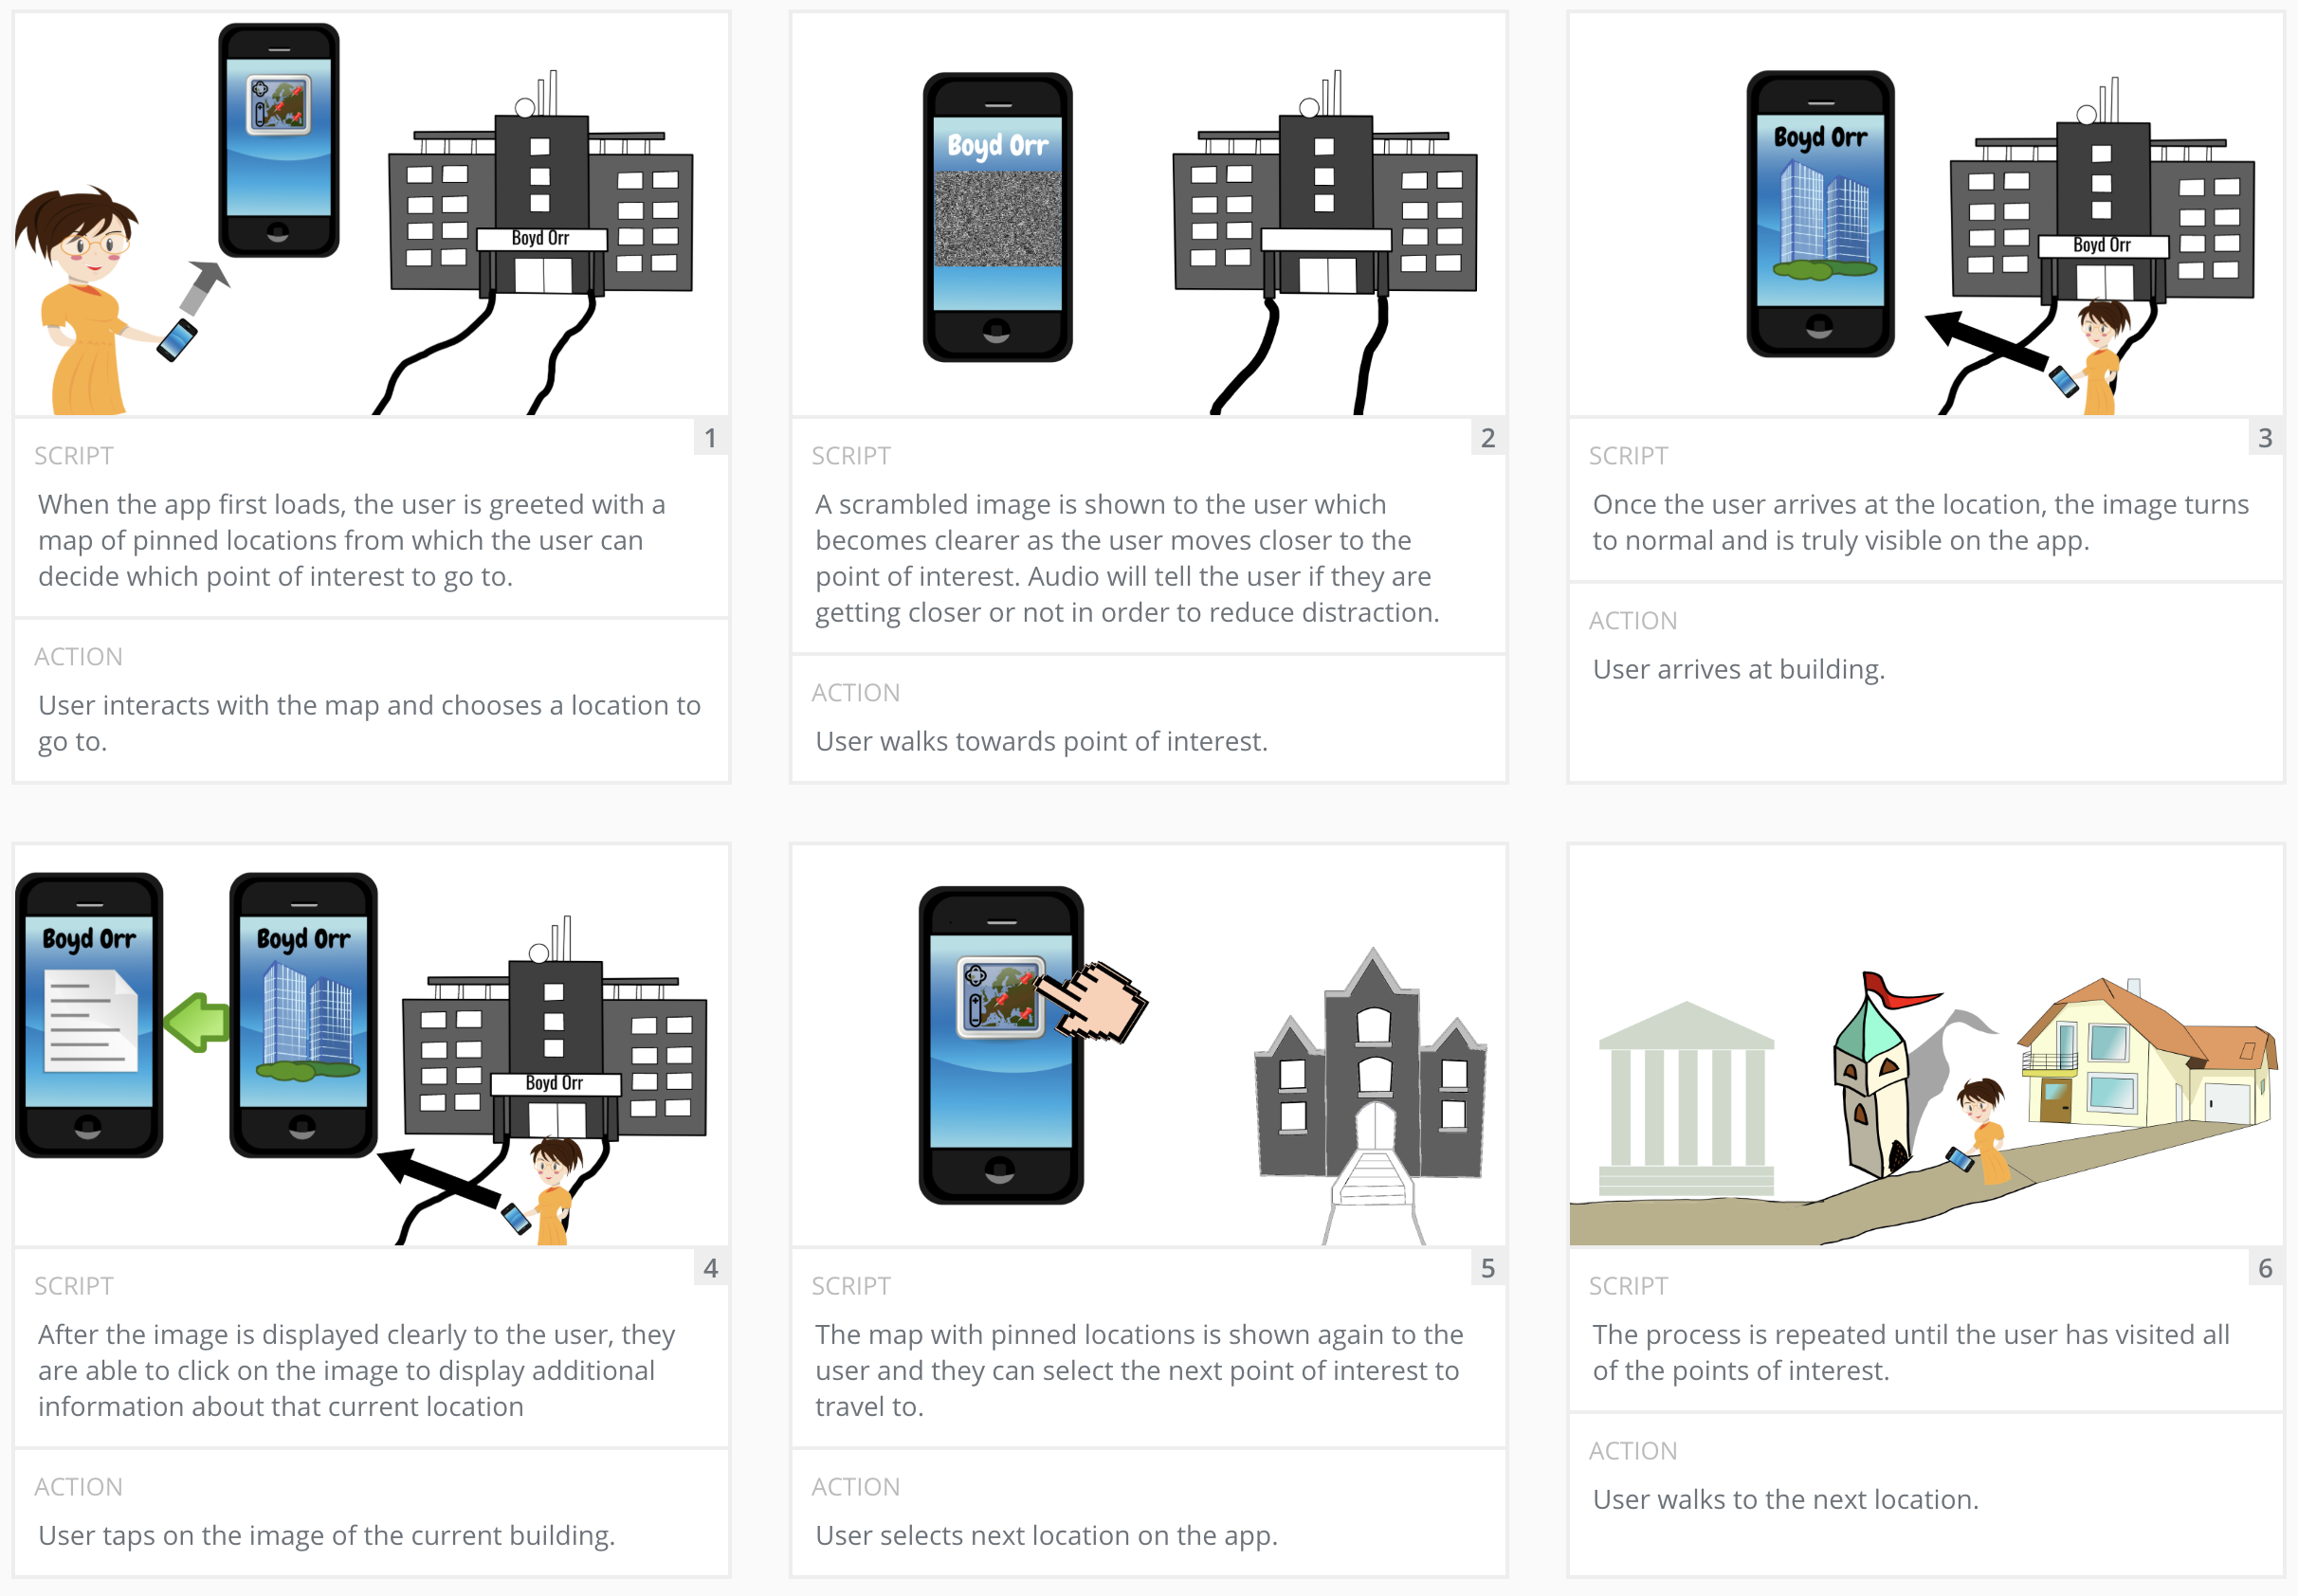
\includegraphics[width=\columnwidth]{storyboard3.png}

\subsection{Initial Prototyping}
\label{app:proto}
\noindent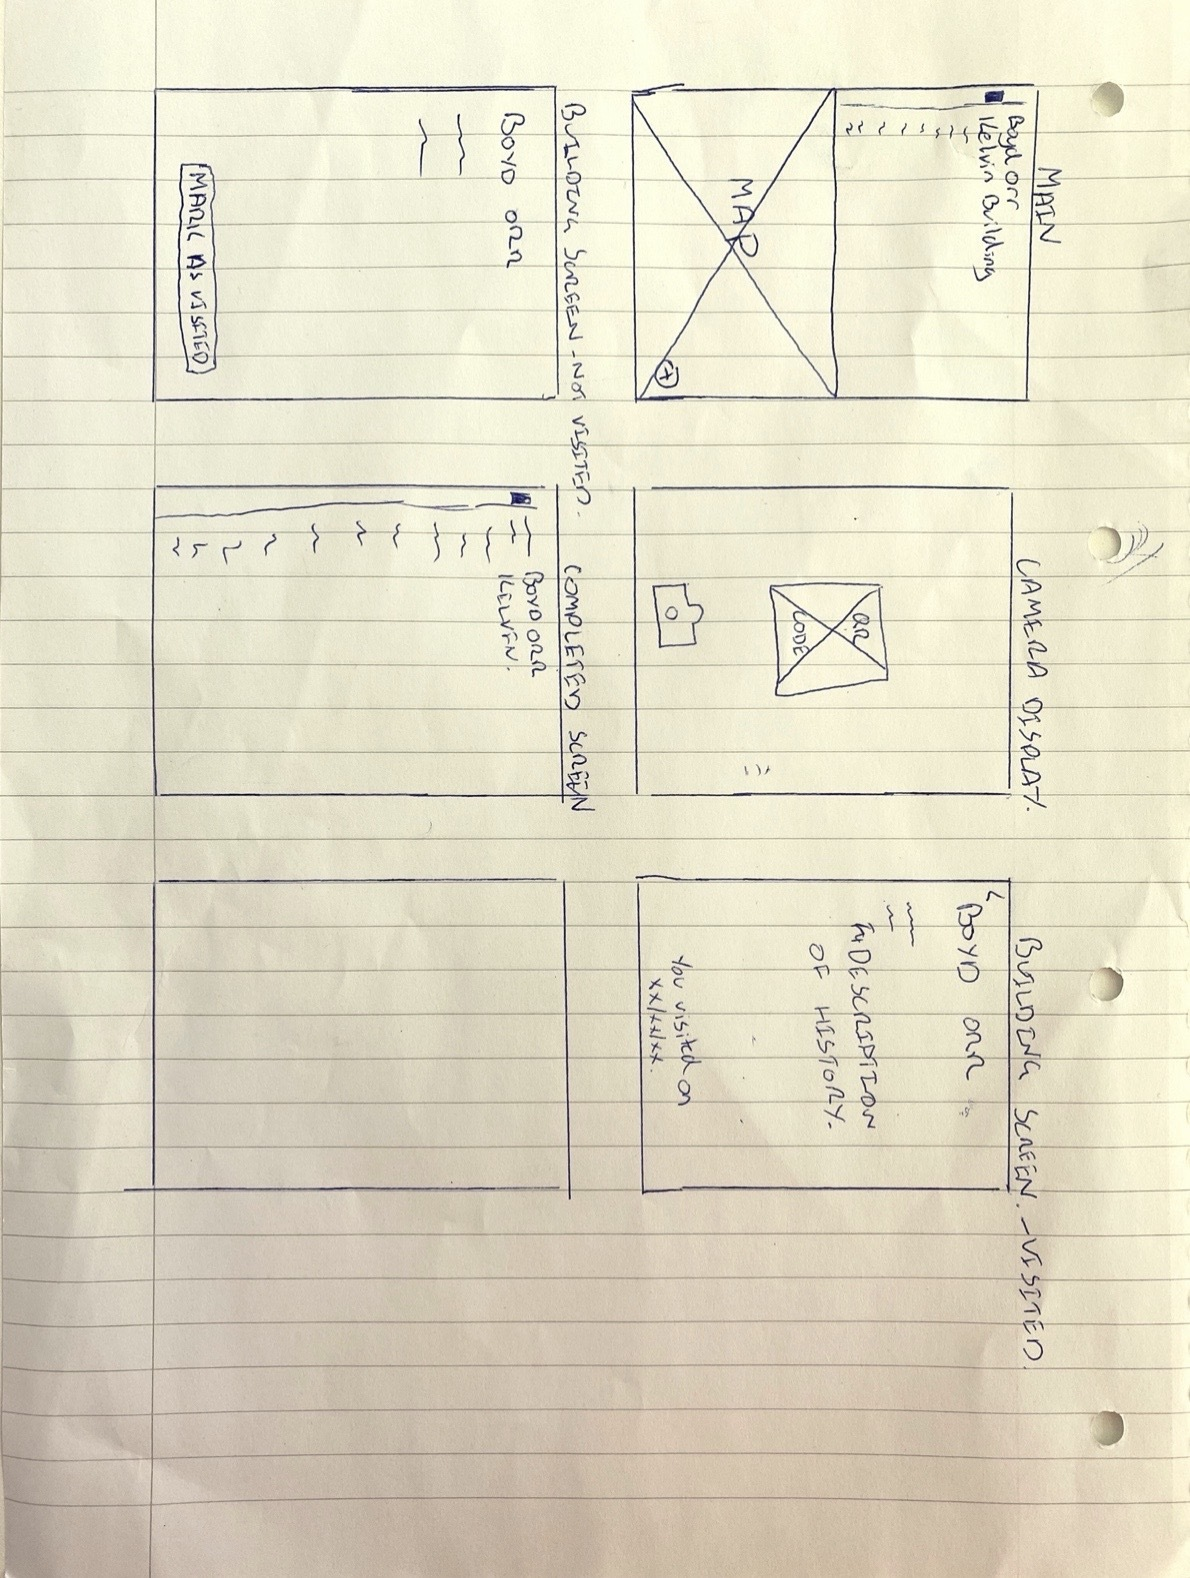
\includegraphics[width=\columnwidth]{paperPrototype1.jpeg}
\noindent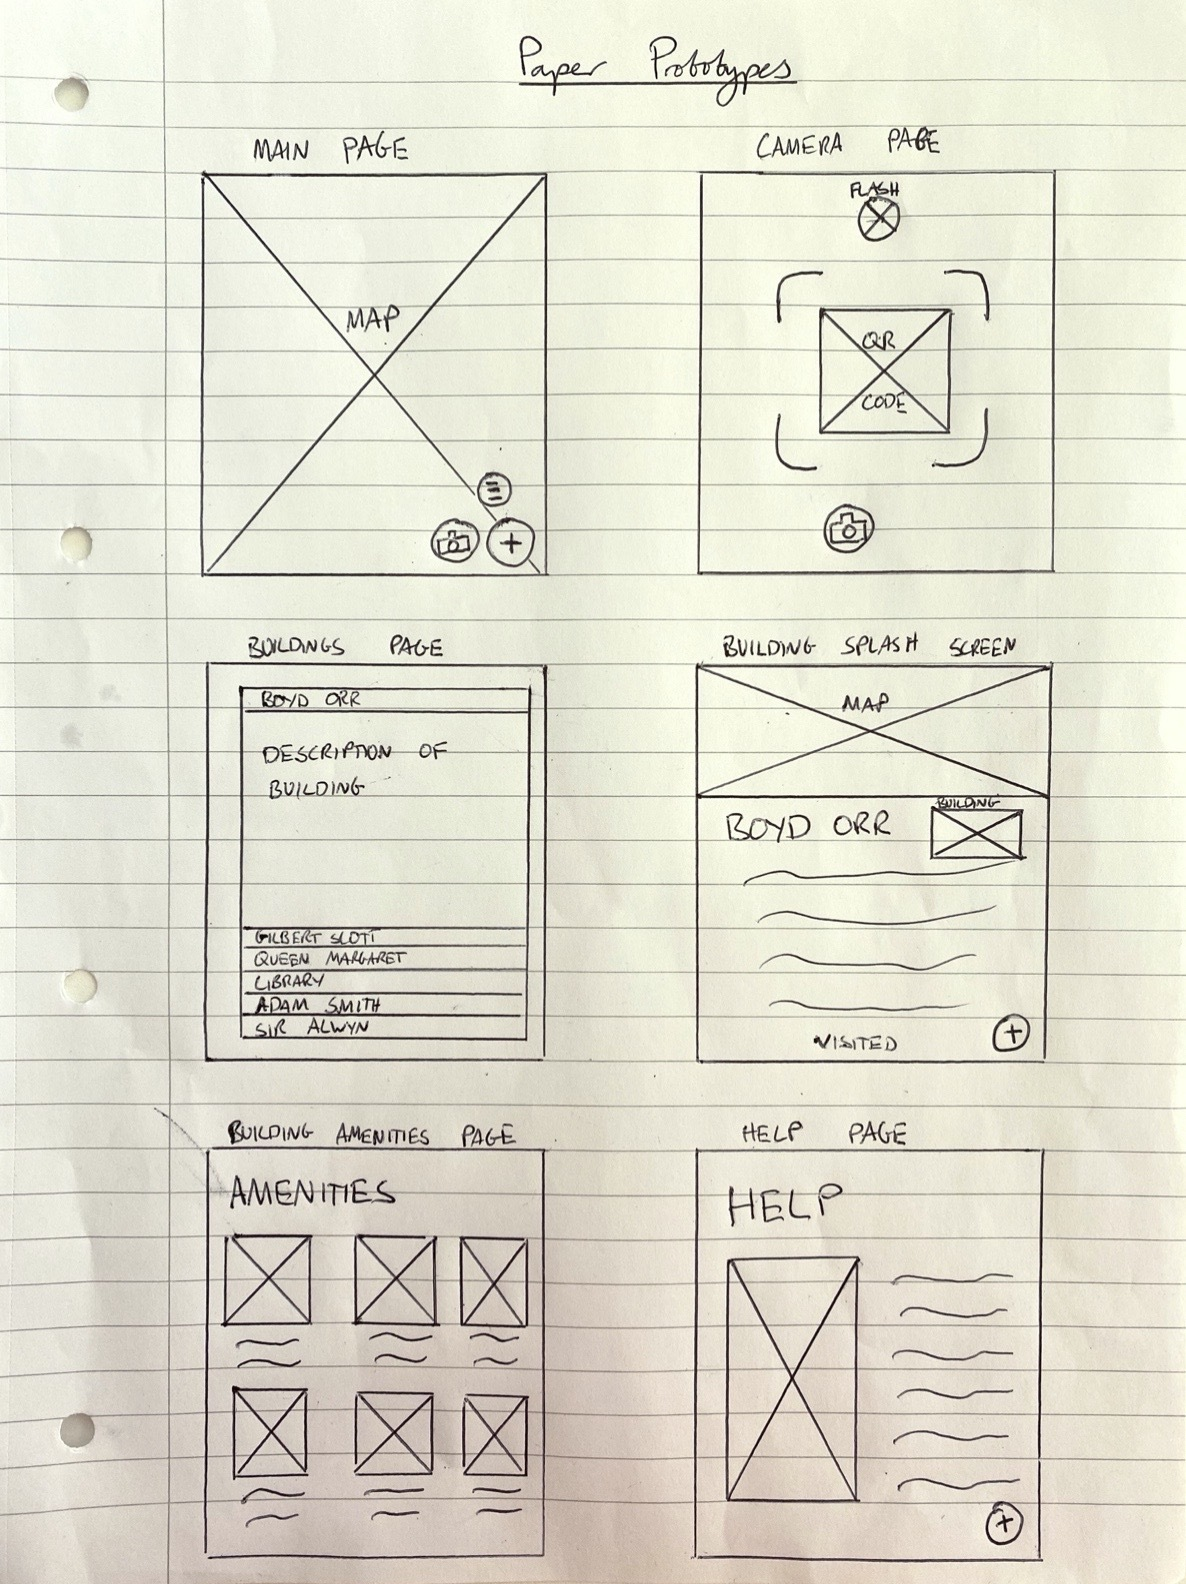
\includegraphics[width=\columnwidth]{paperPrototype2.jpeg}
\noindent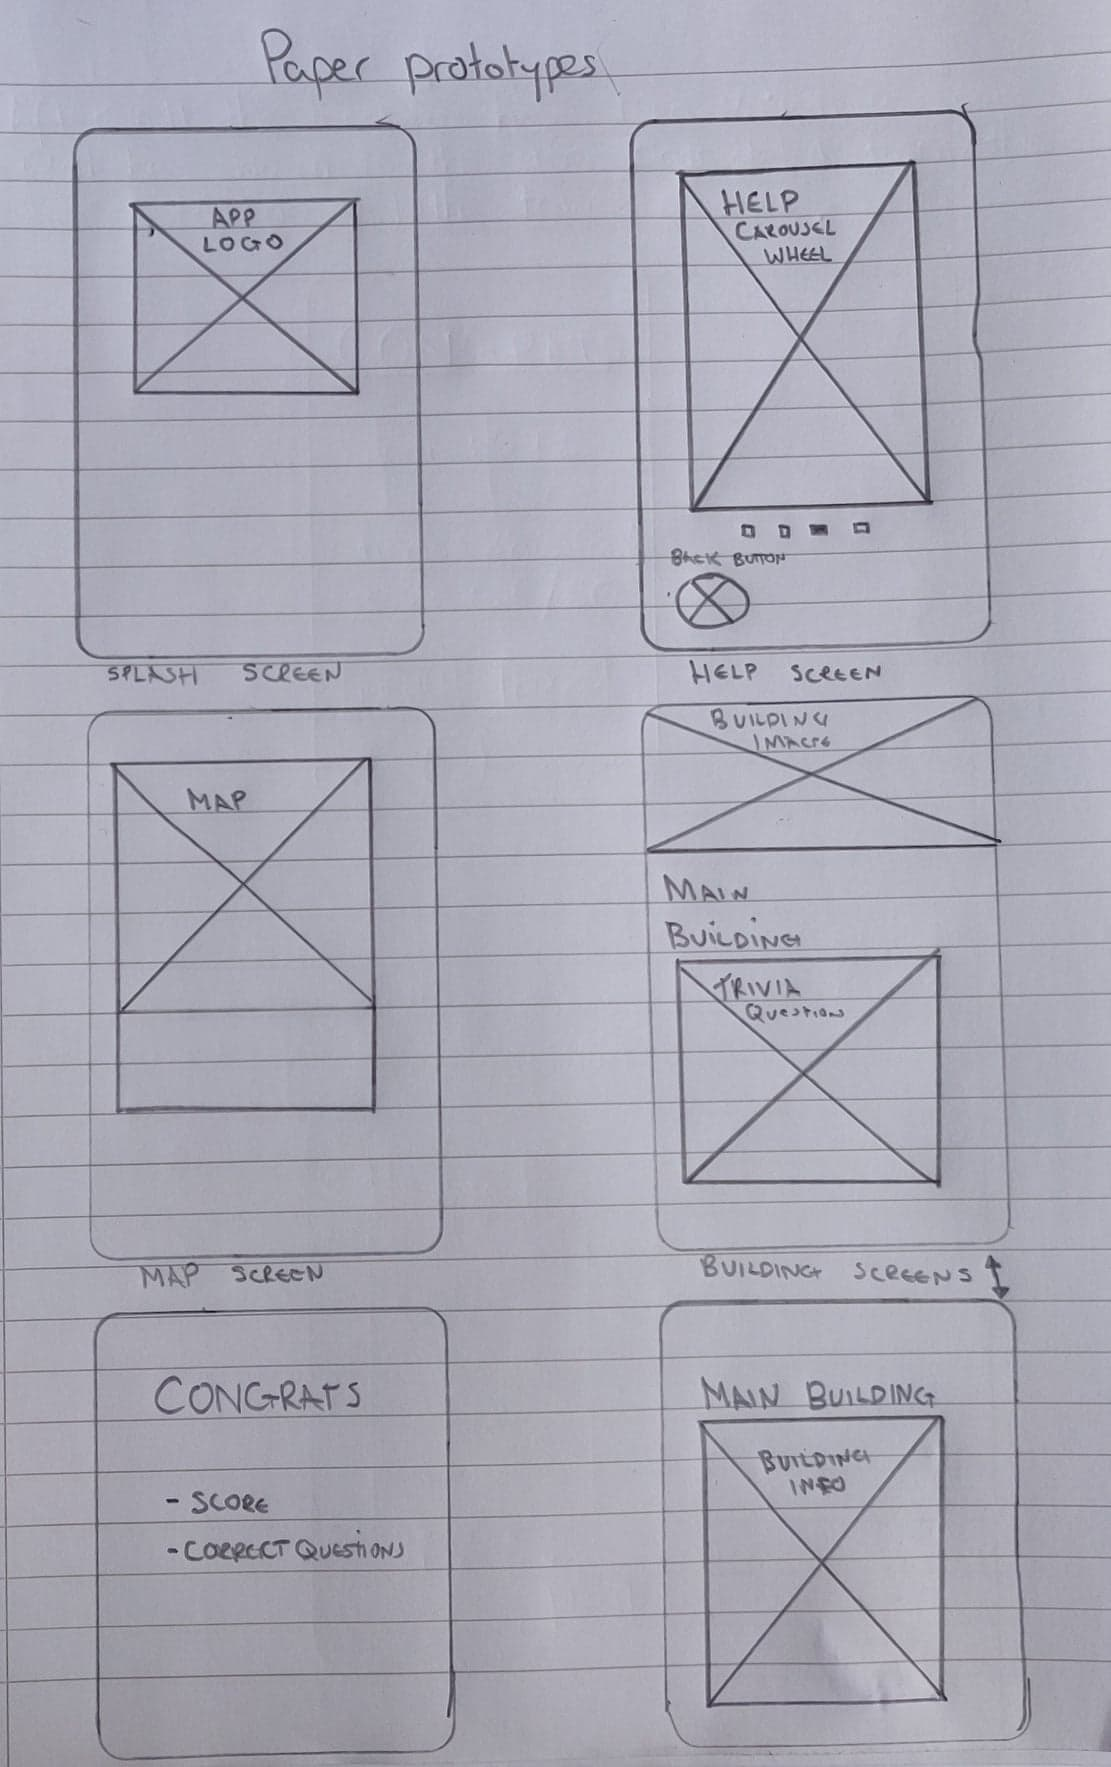
\includegraphics[width=\columnwidth]{paperPrototype3.jpg}

\subsection{Refined Prototyping}
\label{app:refined}
\noindent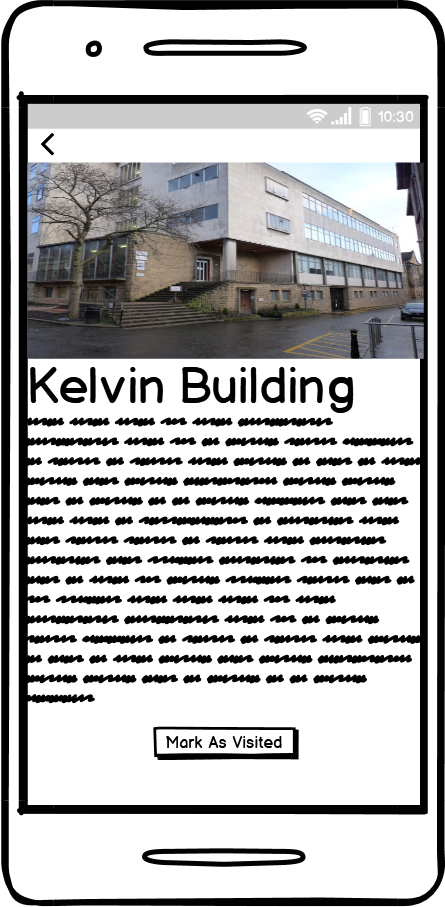
\includegraphics[width=0.6\columnwidth]{refinedPrototype1.png}
\noindent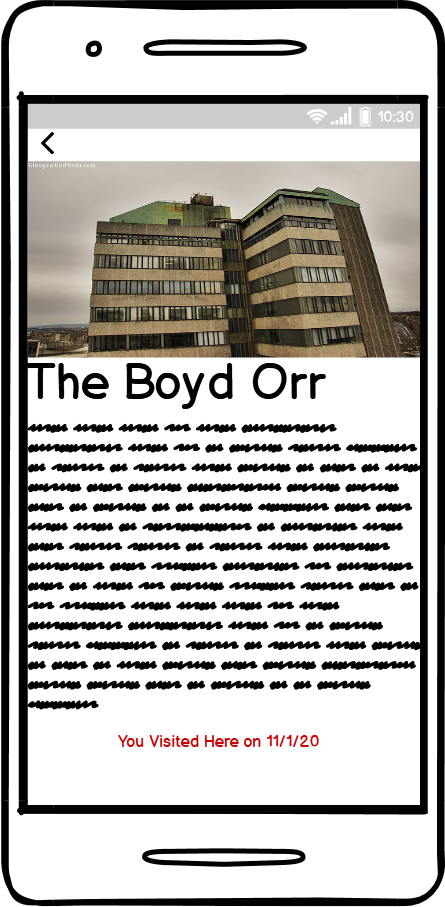
\includegraphics[width=0.6\columnwidth]{refinedPrototype2.png}
\noindent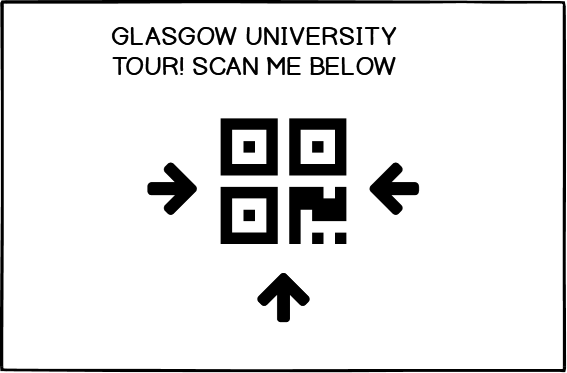
\includegraphics[width=0.6\columnwidth]{refinedPrototype3.png}
\noindent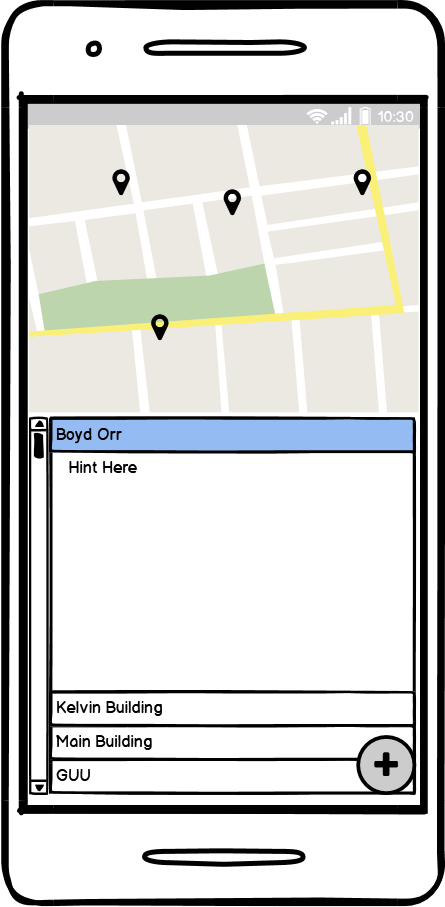
\includegraphics[width=0.6\columnwidth]{refinedPrototype4.png}
\noindent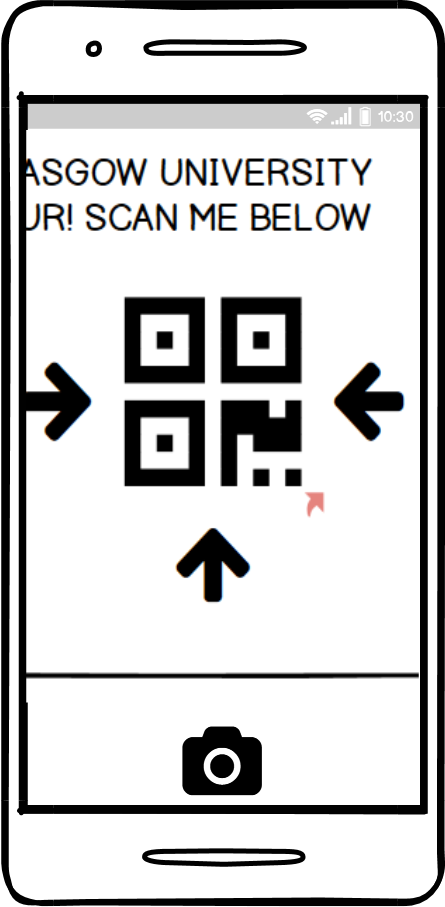
\includegraphics[width=0.6\columnwidth]{refinedPrototype5.png}

\subsection{Evaluation}
\label{appen:eval}
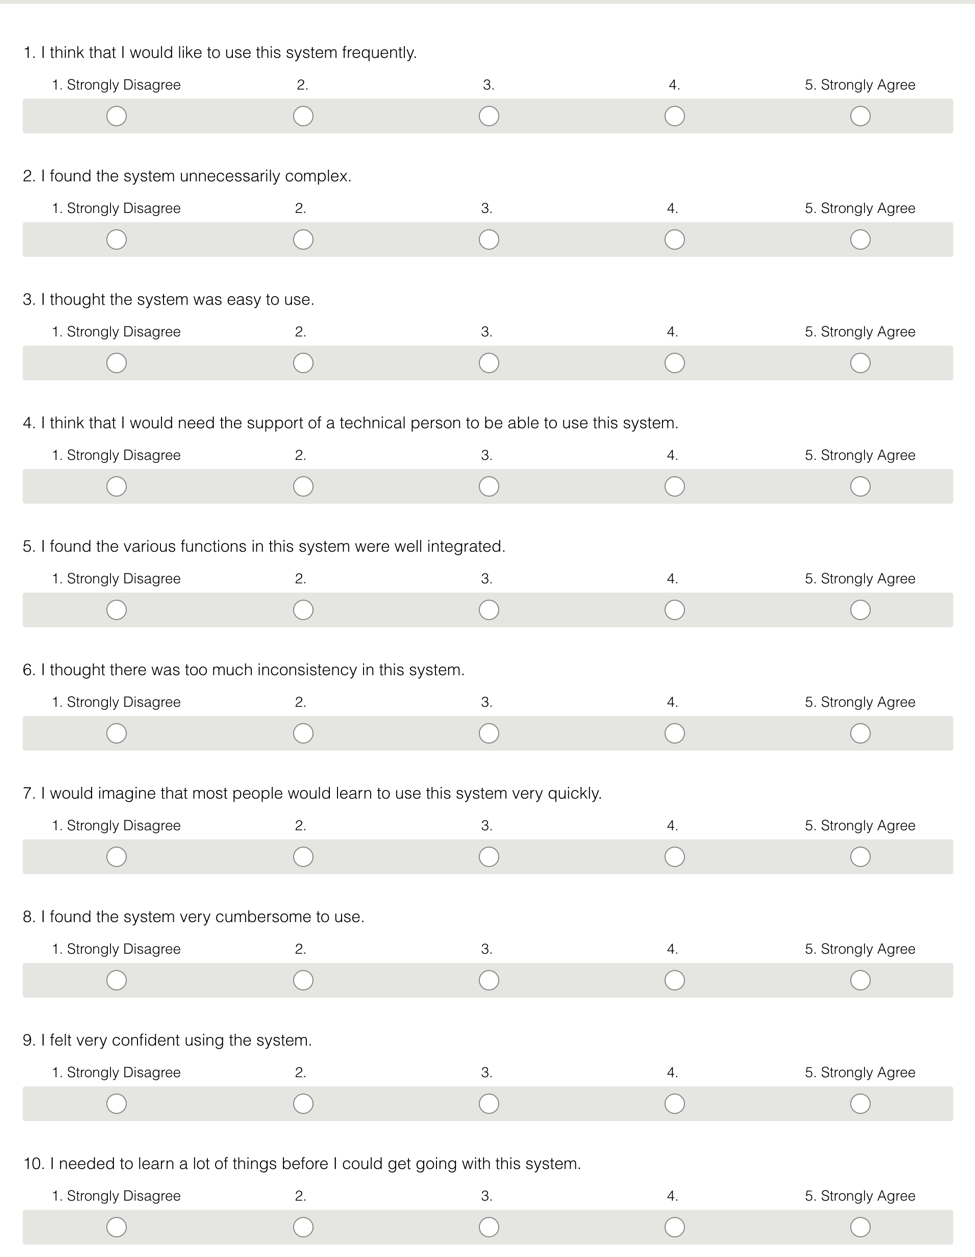
\includegraphics[width=\columnwidth]{sus.png}

\end{document}
